\documentclass[14pt]{extarticle}

\usepackage[table]{xcolor} % colored lines for tables
\usepackage[normalem]{ulem} % strike through text
\usepackage{amsmath,mathtools,amsfonts,amsthm,amssymb,hyperref,pifont}
\usepackage{parskip,geometry,latexsym,bookmark,mathtools,float,cancel}
\usepackage{minted,tcolorbox,bm}

\usepackage[mathscr]{euscript}
\let\euscr\mathscr
\let\mathscr\relax
\usepackage[scr]{rsfso}
\newcommand{\ps}{\mathscr{P}} % for the Power set P

\newtheorem{defn}{Definition}
\newtheorem{thm}{Theorem}
\newtheorem{claim}{Claim}
\newtheorem{lemma}{Lemma}

\newcommand{\dps}{\displaystyle}
\newcommand{\es}{\varnothing}
\newcommand{\fbl}{\underline{\hspace{1cm}}\,\,}
\newcommand{\R}{\mathbb{R}}
\newcommand{\Q}{\mathbb{Q}}
\newcommand{\Z}{\mathbb{Z}}
\newcommand{\from}{\leftarrow}
\newcommand{\true}{{\bf t}}
\newcommand{\false}{{\bf c}}
\newcommand{\bic}{\leftrightarrow}
\newcommand{\da}{\downarrow}
\newcommand{\fa}{\forall}
\newcommand{\te}{\exists}
\newcommand{\cy}{\color{cyan}}

\newcommand{\colsq}[1]{{\color{#1} $\blacksquare$}}

\newcommand{\base}[1]{{\cy #1}} % for log bases
\newcommand{\floor}[1]{{\left\lfloor#1\right\rfloor}}
\newcommand{\ceil}[1]{{\left\lceil#1\right\rceil}}
\newcommand\Ccancel[2][black]{\renewcommand\CancelColor{\color{#1}}\cancel{#2}}
\newcommand\Cbcancel[2][black]{\renewcommand\CancelColor{\color{#1}}\bcancel{#2}}

\renewcommand{\arraystretch}{1.2}

\hypersetup{colorlinks,allcolors=blue,linktoc=all}
\geometry{a4paper}
\geometry{margin=0.42in}

\title{Solutions to Chapter 7, Susanna Epp Discrete Math 5th Edition}

\author{https://github.com/spamegg1}

\begin{document}
\maketitle
\tableofcontents

\section{Exercise Set 7.1}

\subsection{Exercise 1}
Let \(X = \{1, 3, 5\}\) and \(Y = \{s, t, u, v\}\). Define \(f: X \to Y\) by the following arrow diagram.

\begin{figure}[ht!]
\centering
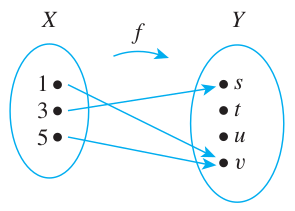
\includegraphics[scale=0.5]{../images/7.1.1.png}
\end{figure}

\subsubsection{(a)}
Write the domain of $f$ and the co-domain of $f$.

\begin{proof}
domain of \(f = \{1, 3, 5\}\), co-domain of \(f = \{s, t, u, v\}\)
\end{proof}

\subsubsection{(b)}
Find $f(1), f(3)$, and $f(5)$.

\begin{proof}
\(f(1) = v, f(3) = s, f(5) = v\)
\end{proof}

\subsubsection{(c)}
What is the range of $f$?

\begin{proof}
range of \(f = \{s, v\}\)
\end{proof}

\subsubsection{(d)}
Is 3 an inverse image of $s$? Is 1 an inverse image of $u$?

\begin{proof}
yes, no
\end{proof}

\subsubsection{(e)}
What is the inverse image of $s$? of $u$? of $v$?

\begin{proof}
inverse image of \(s = \{3\}\), inverse image of \(u = \es\), inverse image of \(v = \{1, 5\}\)
\end{proof}

\subsubsection{(f)}
Represent $f$ as a set of ordered pairs.

\begin{proof}
\(\{(1, v), (3, s), (5, v)\}\)
\end{proof}

\subsection{Exercise 2}
Let \(X = \{1, 3, 5\}\) and \(Y = \{a, b, c, d\}\). Define \(g: X \to Y\) by the following arrow diagram.

\begin{figure}[ht!]
\centering
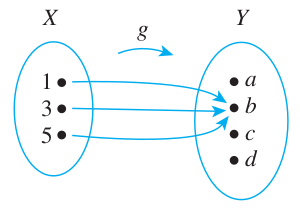
\includegraphics[scale=0.6]{../images/7.1.2.png}
\end{figure}

\subsubsection{(a)}
Write the domain of $g$ and the co-domain of $g$.

\begin{proof}
domain: \(\{1, 3, 5\}\) co-domain: \(\{a,b,c,d\}\)
\end{proof}

\subsubsection{(b)}
Find $g(1), g(3)$, and $g(5)$.

\begin{proof}
\(g(1) = b, g(3) = b, g(5) = b\)
\end{proof}

\subsubsection{(c)}
What is the range of $g$?

\begin{proof}
\(\{b\}\)
\end{proof}

\subsubsection{(d)}
Is 3 an inverse image of $a$? Is 1 an inverse image of $b$?

\begin{proof}
no, yes
\end{proof}

\subsubsection{(e)}
What is the inverse image of $b$? of $c$?

\begin{proof}
\(\{1,3,5\}\) and $\es$
\end{proof}

\subsubsection{(f)}
Represent $g$ as a set of ordered pairs.

\begin{proof}
\(\{(1,b),(3,b),(5,b)\}\)
\end{proof}


\subsection{Exercise 3}
Indicate whether the statements in parts (a)–(d) are true or false for all functions. Justify your answers.

\subsubsection{(a)}
If two elements in the domain of a function are equal, then their images in the co-domain are equal.

\begin{proof}
True. The definition of function says that for any input there is one and only one output, so if two inputs are 
equal, their outputs must also be equal.
\end{proof}

\subsubsection{(b)}
If two elements in the co-domain of a function are equal, then their preimages in the domain are also equal.

\begin{proof}
Not necessarily true. A function can have the same output for more than one input.
\end{proof}

\subsubsection{(c)}
A function can have the same output for more than one input.

\begin{proof}
True. The definition of function does not prohibit this occurrence.
\end{proof}

\subsubsection{(d)}
A function can have the same input for more than one output.

\begin{proof}
False, this is ruled out by the definition of a function. Functions are single valued. Every input corresponds to 
only one output.
\end{proof}

\subsection{Exercise 4}
\subsubsection{(a)}
Find all functions from \(X = \{a, b\}\) to \(Y = \{u, v\}\).

\begin{proof}
There are four functions from $X$ to $Y$ as shown {\it on the next page}.

\begin{figure}[ht!]
\centering
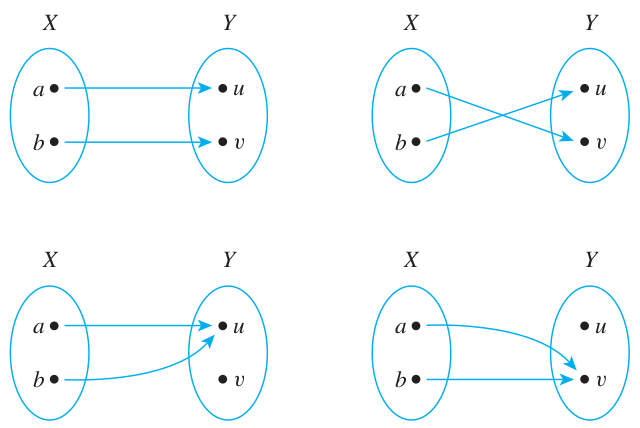
\includegraphics[scale=0.5]{../images/7.1.4.a.png}
\end{figure}

\end{proof}

\subsubsection{(b)}
Find all functions from \(X = \{a, b, c\}\) to \(Y = \{u\}\).

\begin{proof}
There is only one function $f: X \to Y$ given by the set \(\{(a,u), (b,u), (c,u)\}\).
\end{proof}

\subsubsection{(c)}
Find all functions from \(X = \{a, b, c\}\) to \(Y = \{u, v\}\).

\begin{proof}
There are 8 functions:

\(\{(a,u), (b,u), (c,u)\}\)

\(\{(a,u), (b,u), (c,v)\}\)

\(\{(a,u), (b,v), (c,u)\}\)

\(\{(a,u), (b,v), (c,v)\}\)

\(\{(a,v), (b,u), (c,u)\}\)

\(\{(a,v), (b,u), (c,v)\}\)

\(\{(a,v), (b,v), (c,u)\}\)

\(\{(a,v), (b,v), (c,v)\}\)
\end{proof}

\subsection{Exercise 5}
Let $I_{\Z}$ be the identity function defined on the set of all integers, and suppose that \(e, b_{i}^{jk}, K(t)\), and 
\(u_{kj}\) all represent integers. Find the following:

\subsubsection{(a)}
\(I_{\Z}(e)\)

\begin{proof}
$e$ (because \(I_{\Z}\) is the identity function).
\end{proof}

\subsubsection{(b)}
\(I_{\Z}(b_{i}^{jk})\)

\begin{proof}
$b_{i}^{jk}$ (because \(I_{\Z}\) is the identity function).
\end{proof}

\subsubsection{(c)}
\(I_{\Z}(K(t))\)

\begin{proof}
$K(t)$ (because \(I_{\Z}\) is the identity function).
\end{proof}

\subsubsection{(d)}
\(I_{\Z}(u_{kj})\)

\begin{proof}
$u_{kj}$ (because \(I_{\Z}\) is the identity function).
\end{proof}

\subsection{Exercise 6}
Find functions defined on the set of nonnegative integers that can be used to define the sequences whose first six 
terms are given below.

\subsubsection{(a)}
\(\dps 1, -\frac{1}{3}, \frac{1}{5}, -\frac{1}{7}, \frac{1}{9}, -\frac{1}{11}\)

\begin{proof}
The sequence is given by the function \(f: \Z^{nonneg} \to \R\) defined by the rule \(\dps f(n)=\frac{(-1)^n}{2n+1}\)
{\cy for each nonnegative integer $n$.}
\end{proof}

\subsubsection{(b)}
\(0, -2, 4, -6, 8, -10\)

\begin{proof}
The sequence is given by the function \(f: \Z^{nonneg} \to \Z\) defined by the rule \(\dps f(n) = (-1)^n \cdot (2n)\)
{\cy for each nonnegative integer $n$.}
\end{proof}

\subsection{Exercise 7}
Let \(A = \{1, 2, 3, 4, 5\}\), and define a function \(F: \ps(A) \to \Z\) as follows: For each set $X$ in $\ps(A)$,
\[
F(x) =
\left\{
\begin{tabular}{ll}
\(0\) & if $X$ has an even number of elements \\
\(1\) & if $X$ has an odd number of elements
\end{tabular}
\right.
\]
Find the following:

\subsubsection{(a)}
\(F(\{1, 3, 4\})\) 

\begin{proof}
\(F(\{1, 3, 4\}) = 1\) {\it [because \(\{1, 3, 4\}\) has an odd number of elements]}

\end{proof}

\subsubsection{(b)}
\(F(\es)\)

\begin{proof}
\(F(\{\es\}) = 0\) {\it [because \(\{\es\}\) has an even number of elements]}
\end{proof}

\subsubsection{(c)}
\(F(\{2, 3\})\)

\begin{proof}
\(F(\{2, 3\}) = 0\) {\it [because \(\{2, 3\}\) has an even number of elements]}
\end{proof}

\subsubsection{(d)}
\(F(\{2, 3, 4, 5\})\)

\begin{proof}
\(F(\{2, 3, 4, 5\}) = 0\) {\it [because \(\{2, 3, 4, 5\}\) has an even number of elements]}
\end{proof}

\subsection{Exercise 8}
Let \(J_5 = \{0, 1, 2, 3, 4\}\), and define a function \(F: J_5 \to J_5\) as follows: For each \(x \in J_5, F(x) = (x^3 
+ 2x + 4) \mod 5\). Find the following:

\subsubsection{(a)}
$F(0)$

\begin{proof}
\(F(0) = (0^3 + 2 \cdot 0 + 4) \mod 5 = 4 \mod 5 = 4\)

\end{proof}

\subsubsection{(b)}
$F(1)$

\begin{proof}
\(F(1) = (1^3 + 2 \cdot 1 + 4) \mod 5 = 7 \mod 5 = 2\)
\end{proof}

\subsubsection{(c)}
$F(2)$

\begin{proof}
\(F(2) = (2^3 + 2 \cdot 2 + 4) \mod 5 = 16 \mod 5 = 1\)
\end{proof}

\subsubsection{(d)}
$F(3)$

\begin{proof}
\(F(3) = (3^3 + 2 \cdot 3 + 4) \mod 5 = 37 \mod 5 = 2\)
\end{proof}

\subsubsection{(e)}
$F(4)$

\begin{proof}
\(F(4) = (4^3 + 2 \cdot 4 + 4) \mod 5 = 76 \mod 5 = 1\)
\end{proof}

\subsection{Exercise 9}
Define a function \(S: \Z^+ \to \Z^+\) as follows: For each positive integer \(n, S(n) =\) the sum of the positive 
divisors of $n$. Find the following:

\subsubsection{(a)}
$S(1)$

\begin{proof}
$S(1) = 1$

\end{proof}

\subsubsection{(b)}
$S(15)$

\begin{proof}
\(S(15) = 1 + 3 + 5 + 15 = 24\)
\end{proof}

\subsubsection{(c)}
$S(17)$

\begin{proof}
\(S(15) = 1 + 17 = 18\)
\end{proof}

\subsubsection{(d)}
$S(5)$

\begin{proof}
\(S(5) = 1 + 5 = 6\)
\end{proof}

\subsubsection{(e)}
$S(18)$

\begin{proof}
\(S(18) = 1 + 2 + 3 + 6 + 9 + 18 = 39\)
\end{proof}

\subsubsection{(f)}
$S(21)$

\begin{proof}
\(S(21) = 1 + 3 + 7 + 21 = 32\)
\end{proof}

\subsection{Exercise 10}
Let $D$ be the set of all finite subsets of positive integers. Define a function \(T: \Z^+ \to D\) as follows: 
For each positive integer \(n, T(n) =\) the set of positive divisors of $n$. Find the following:

\subsubsection{(a)}
$T(1)$

\begin{proof}
\(T(1) = \{1\}\)

\end{proof}

\subsubsection{(b)}
$T(15)$

\begin{proof}
\(T(15) = \{1, 3, 5, 15\}\)
\end{proof}

\subsubsection{(c)}
$T(17)$

\begin{proof}
\(T(17) = \{1, 17\}\)
\end{proof}

\subsubsection{(d)}
$T(5)$

\begin{proof}
\(T(1) = \{1\}\)
\end{proof}

\subsubsection{(e)}
$T(18)$

\begin{proof}
\(T(18) = \{1, 2, 3, 6, 9, 18\}\)
\end{proof}

\subsubsection{(f)}
$T(21)$

\begin{proof}
\(T(21) = \{1, 3, 7, 21\}\)
\end{proof}

\subsection{Exercise 11}
Define \(F: \Z \times \Z \to \Z \times \Z\) as follows: For every ordered pair \((a,b)\) of integers, \(F(a,b) = (2a+1, 
3b-2)\). Find the following:

\subsubsection{(a)}
$F(4,4)$

\begin{proof}
\(F(4, 4) = (2 \cdot 4 + 1, 3 \cdot 4 - 2) = (9, 10)\)
\end{proof}

\subsubsection{(b)}
$F(2,1)$

\begin{proof}
\(F(2, 1) = (2 \cdot 2 + 1, 3 \cdot 1 - 2) = (5, 1)\)
\end{proof}

\subsubsection{(c)}
$F(3,2)$

\begin{proof}
\(F(3, 3) = (2 \cdot 3 + 1, 3 \cdot 3 - 2) = (7, 7)\)
\end{proof}

\subsubsection{(d)}
$F(1,5)$

\begin{proof}
\(F(1, 5) = (2 \cdot 1 + 1, 3 \cdot 5 - 2) = (3, 13)\)
\end{proof}

\subsection{Exercise 12}
Let \(J_5 = \{0, 1, 2, 3, 4\}\), and define \(G: J_5 \times J_5 \to J_5 \times J_5\) as follows: For each \((a,b) \in 
J_5 \times J_5, G(a,b) = ((2a+1) \mod 5, (3b-2) \mod 5)\). Find the following:

\subsubsection{(a)}
$G(4,4)$

\begin{proof}
\(G(4, 4) = ((2 \cdot 4 + 1) \mod 5, (3 \cdot 4 - 2) \mod 5) = (9 \mod 5, 10 \mod 5) = (4, 0)\)
\end{proof}

\subsubsection{(b)}
$G(2,1)$

\begin{proof}
\(G(2, 1) = ((2 \cdot 2 + 1) \mod 5, (3 \cdot 1 - 2) \mod 5) = (5 \mod 5, 1 \mod 5) = (0, 1)\)
\end{proof}

\subsubsection{(c)}
$G(3,2)$

\begin{proof}
\(G(3, 2) = ((2 \cdot 3 + 1) \mod 5, (3 \cdot 2 - 2) \mod 5) = (7 \mod 5, 4 \mod 5) = (2, 4)\)
\end{proof}

\subsubsection{(d)}
$G(1,5)$

\begin{proof}
\(G(1, 5) = ((2 \cdot 1 + 1) \mod 5, (3 \cdot 5 - 2) \mod 5) = (3 \mod 5, 13 \mod 5) = (3, 3)\)
\end{proof}

\subsection{Exercise 13}
Let \(J_5 = \{0, 1, 2, 3, 4\}\), and define functions \(f: J_5 \to J_5\) and \(g: J_5 \to J_5\) as follows: For each 
\(x \in J_5, f(x) = (x + 4)^2 \mod 5\) and \(g(x) = (x^2 + 3x + 1) \mod 5\). Is $f = g$? Explain.

\begin{proof}
\begin{center}
\arrayrulecolor{cyan}
\begin{tabular}{|c|c|c|}
\hline
$x$ & $f(x)$ & $g(x)$ \\
\hline
0 & \(4^2 \mod 5 = 1\) & \((0^2 + 3 \cdot 0 + 1) \mod 5 = 1\) \\
\hline
1 & \(5^2 \mod 5 = 0\) & \((1^2 + 3 \cdot 1 + 1) \mod 5 = 0\) \\
\hline
2 & \(6^2 \mod 5 = 1\) & \((2^2 + 3 \cdot 2 + 1) \mod 5 = 1\) \\
\hline
3 & \(7^2 \mod 5 = 4\) & \((3^2 + 3 \cdot 3 + 1) \mod 5 = 4\) \\
\hline
4 & \(8^2 \mod 5 = 4\) & \((4^2 + 3 \cdot 4 + 1) \mod 5 = 4\) \\
\hline
\end{tabular}
\arrayrulecolor{black}
\end{center}

The table shows that \(f(x) = g(x)\) for every $x$ in \(J_5\). Thus, by definition of equality of functions, $f = g$.
\end{proof}

\subsection{Exercise 14}
Define functions $H$ and $K$ from $\R$ to $\R$ by the following formulas: For every \(x \in \R, H(x) = \floor{x} 
+ 1\) and \(K(x) = \ceil{x}\). Does $H = K$? Explain.

\begin{proof}
No, because \(H(2) = \floor{2} + 1 = 3 \neq 2 = \ceil{2} = K(2)\).
\end{proof}

\subsection{Exercise 15}
Let $F$ and $G$ be functions from the set of all real numbers to itself. Define new functions 
\(F \cdot G: \R \to \R\) and \(G \cdot F: \R \to \R\) as follows: For every \(x \in \R\), 
\((F \cdot G)(x) = F(x) \cdot G(x)\), \((G \cdot F)(x) = G(x) \cdot F(x)\). Does $F \cdot G = G \cdot F$? Explain.

\begin{proof}
\begin{tabular}{rcll}
\((F \cdot G)(x)\) & = & \(F(x) \cdot G(x)\) & {\cy by definition of $F \cdot G$} \\
& = & \(G(x) \cdot F(x)\) & {\cy by commutative law for real numbers} \\
& = & \((G \cdot F)(x)\) & {\cy by definition of $G \cdot F$}
\end{tabular}

for every real number $x$. Therefore $F\cdot G$ and $G \cdot F$ are equal.
\end{proof}

\subsection{Exercise 16}
Let $F$ and $G$ be functions from the set of all real numbers to itself. Define new functions 
\(F - G: \R \to \R\) and \(G - F: \R \to \R\) as follows: For every \(x \in \R\), \((F - G)(x) = F(x) - G(x)\), 
\((G - F)(x) = G(x) - F(x)\). Does $F - G = G - F$? Explain.

\begin{proof}
\underline{Counterexample:} Let \(F(x) = 2x, G(x) = 3x\). 
Then 
\[
(F-G)(1) = F(1) - G(1) = 2 - 3 = -1 \neq 1 = 3 - 2 = G(1) - F(1) = (G-F)(1).
\] 
Therefore $F - G$ does not equal $G - F$.
\end{proof}

\subsection{Exercise 17}
Use the definition of logarithm to fill in the blanks below.

\subsubsection{(a)}
\(\log_{2} 8 = 3\) because \fbl.

\begin{proof}
\(2^3 = 8\)
\end{proof}

\subsubsection{(b)}
\(\log_{5}(\frac{1}{25}) = -2\) because \fbl.

\begin{proof}
\(\dps 5^{-2} = \frac{1}{25}\)
\end{proof}

\subsubsection{(c)}
\(\log_{4} 4 = 1\) because \fbl.

\begin{proof}
\(4^1 = 4\)
\end{proof}

\subsubsection{(d)}
\(\log_{3}(3^n) = n\) because \fbl.

\begin{proof}
\(3^n = 3^n\)
\end{proof}

\subsubsection{(e)}
\(\log_{4} 1 = 0\) because \fbl.

\begin{proof}
\(4^0 = 1\)
\end{proof}

\subsection{Exercise 18}
Find exact values for each of the following quantities without using a calculator.

\subsubsection{(a)}
\(\log_{3} 81\)

\begin{proof}
4
\end{proof}

\subsubsection{(b)}
\(\log_{2} 1024\)

\begin{proof}
10
\end{proof}

\subsubsection{(c)}
\(\log_{3} \frac{1}{27}\)

\begin{proof}
$-3$
\end{proof}

\subsubsection{(d)}
\(\log_{2} 1\)

\begin{proof}
0
\end{proof}

\subsubsection{(e)}
\(\log_{10}(\frac{1}{10})\)

\begin{proof}
$-1$
\end{proof}

\subsubsection{(f)}
\(\log_{3} 3\)

\begin{proof}
1
\end{proof}

\subsubsection{(g)}
\(\log_{2} 2^k\)

\begin{proof}
$k$
\end{proof}

\subsection{Exercise 19}
Use the definition of logarithm to prove that for any positive real number $b$ with \(b \neq 1, \log_b b = 1\).

\begin{proof}
Let $b$ be any positive real number with \(b \neq 1\). Since \(b^1 = b\), then \(\log_b b = 1\) by definition of logarithm.
\end{proof}

\subsection{Exercise 20}
Use the definition of logarithm to prove that for any positive real number $b$ with \(b \neq 1, \log_b 1 = 0\).

\begin{proof}
Let $b$ be any positive real number with \(b \neq 1\). Since \(b^0 = 1\), then \(\log_b 1 = 0\) by definition of logarithm.
\end{proof}

\subsection{Exercise 21}
If $b$ is any positive real number with \(b \neq 1\) and $x$ is any real number, \(b^{-x}\) is defined as follows: 
\(\dps b^{-x} = \frac{1}{b^x}\). Use this definition and the definition of logarithm to prove that \(\dps \log_b 
\left(\frac{1}{u}\right) = -\log_b(u)\) for all positive real numbers $u$ and $b$, with \(b \neq 1\).

\begin{proof}
Suppose $b$ and $u$ are any positive real numbers with \(b \neq 1\). {\it [We must show that \(\log_b (\frac{1}{u}) = 
-\log_b(u)\).]} Let \(v = \log_b (\frac{1}{u})\). By definition of logarithm, \(b^v = \frac{1}{u}\). Multiplying 
both sides by $u$ and dividing by $b^v$ gives \(u=b^{-v}\), and thus, by definition of logarithm, \(-v = \log_b(u)\). 
When both sides of this equation are multiplied by $-1$, the result is \(v = -\log_b(u)\). Therefore, \(\log_b 
(\frac{1}{u}) = - \log_b(u)\) because both expressions equal $v$. {\it [This is what was to be shown.]}
\end{proof}

\subsection{Exercise 22}
Use the unique factorization for the integers theorem (Section 4.4) and the definition of logarithm to prove that 
$\log_3(7)$ is irrational.

\begin{proof}
1. Argue by contradiction and assume \(r = \log_3(7)\) is rational.

2. By 1 and definition of rational, \(r = a / b\) for some integers $a,b$ where $b \neq 0$.

3. We may assume \(b > 0\). (If \(b < 0\) then \(a/b = (-a)/(-b)\) therefore we can replace $a/b$ with $-a/(-b)$
where \(-b > 0\).)

4. By 1, 2 and definition of logarithm, \(7 = 3^{a/b}\).

5. By 4, taking the $b$th powers of both sides, we get \(7^b = 3^a\).

6. Since \(b\) is a positive integer, \(7^b\) is a positive integer. Therefore \(3^a\) is the same positive integer.

7. By 6, we have two different prime factorizations of the same positive integer. By the uniqueness part of the prime
factorization theorem, this is only possible if the positive integer is equal to 1.

8. By 7, \(7^b = 3^a = 1\) so \(a = b = 0\). This is a contradiction since \(b > 0\).

9. So our supposition in 1 is false by 8, thus \(\log_3(7)\) is irrational.
\end{proof}

\subsection{Exercise 23}
If $b$ and $y$ are positive real numbers such that \(\log_b y = 3\), what is \(\log_{1/b}(y)\)? Explain.

\begin{proof}
By definition of logarithm with base $b$, \(b^3 = y\). So
\[
y = b^3 = \frac{1}{\frac{1}{b^3}} = \frac{1}{\left(\frac{1}{b}\right)^3} = \left(\frac{1}{b}\right)^{-3}
\]
So by definition of logarithm with base $1/b$, \(\log_{1/b}(y) = -3\).
\end{proof}

\subsection{Exercise 24}
If $b$ and $y$ are positive real numbers such that \(\log_b y = 2\), what is \(\log_{b^2}(y)\)? Explain.

\begin{proof}
By definition of logarithm with base $b$, \(b^2 = y\). So
by definition of logarithm with base $b^2$, 
\(\log_{b^2}(y) = 1\) because \((b^2)^1 = y\).
\end{proof}

\subsection{Exercise 25}
Let \(A = \{2, 3, 5\}\) and \(B = \{x, y\}\). Let $p_1$ and $p_2$ be the projections of \(A \times B\) onto the first 
and second coordinates. That is, for each pair \((a, b) \in A \times B, p_1(a, b) = a\) and \(p_2(a, b) = b\).

\subsubsection{(a)}
Find \(p_1(2, y)\) and \(p_1(5, x)\). What is the range of $p_1$?

\begin{proof}
\(p_1(2, y) = 2, p_1(5, x) = 5\), range of \(p_1 = \{2, 3, 5\}\)
\end{proof}

\subsubsection{(b)}
Find \(p_2(2, y)\) and \(p_2(5, x)\). What is the range of $p_2$?

\begin{proof}
\(p_2(2, y) = y, p_2(5, x) = x\), range of \(p_2 = \{x, y\}\)
\end{proof}

\subsection{Exercise 26}
Observe that mod and div can be defined as functions from \(\Z^{nonneg} \times \Z^+\) to $\Z$. For each ordered pair 
\((n, d)\) consisting of a nonnegative integer $n$ and a positive integer $d$, let

\(mod(n, d) = n \mod d\) (the nonnegative remainder obtained when $n$ is divided by $d$).

\(div(n, d) = n \text{ div } d\) (the integer quotient obtained when $n$ is divided by $d$).

Find each of the following:

\subsubsection{(a)}
\(mod(67, 10)\) and \(div(67, 10)\)

\begin{proof}
\(mod(67, 10) = , div(67, 10) = \)
\end{proof}

\subsubsection{(b)}
$mod(59, 8)$ and $div(59, 8)$

\begin{proof}
\(mod(67, 10) = 7, div(67, 10) = 6\)
\end{proof}

\subsubsection{(c)}
$mod(30, 5)$ and $div(30, 5)$

\begin{proof}
\(mod(30, 5) = 0, div(30, 5) = 6\)
\end{proof}

\subsection{Exercise 27}
Let $S$ be the set of all strings of $a$’s and $b$’s.

\subsubsection{(a)}
Define \(f: S \to \Z\) as follows: For each string $s$ in $S$
\[
f(s) =
\left\{
\begin{tabular}{lr}
the number of $b$'s to the left of the left most $a$ in $s$ & if $s$ contains some $a$'s \\
0 & if $s$ contains no $a$'s
\end{tabular}
\right.
\]
Find \(f(aba), f(bbab)\), and \(f(b)\). What is the range of $f$?

\begin{proof}
\(f(aba) = 0\) {\it [because there are no $b$'s to the left
of the leftmost $a$ in $aba$]}

\(f(bbab) = 2\) {\it [because there are two $b$'s to the left of the leftmost $a$ in $bbab$]}

\(f(b) = 0\) {\it [because the string $b$ contains no $a$'s]}

range of \(f = \Z^{nonneg}\)
\end{proof}

\subsubsection{(b)}
Define \(g: S \to S\) as follows: For each string $s$ in $S$, \(g(s) =\) the string obtained by writing the 
characters of $s$ in reverse order. Find \(g(aba), g(bbab)\), and \(g(b)\). What is the range of $g$?

\begin{proof}
\(g(aba) = aba, g(bbab) = babb, g(b) = b\), range of \(g = S\)
\end{proof}

\subsection{Exercise 28}
Consider the coding and decoding functions $E$ and $D$ defined in Example 7.1.9.

\subsubsection{(a)}
Find \(E(0110)\) and \(D(111111000111)\).

\begin{proof}
\(E(0110) = 000111111000\) and \(D(111111000111) = 1101\)
\end{proof}

\subsubsection{(b)}
Find \(E(1010)\) and \(D(000000111111)\).

\begin{proof}
\(E(1010) = 111000111000\) and \(D(000000111111) = 0011\)
\end{proof}

\subsection{Exercise 29}
Consider the Hamming distance function defined in Example 7.1.10.

\subsubsection{(a)}
Find \(H(10101, 00011)\).

\begin{proof}
\(H(10101, 00011)\) = 3
\end{proof}

\subsubsection{(b)}
Find \(H(00110, 10111)\).

\begin{proof}
\(H(00110, 10111)\) = 2
\end{proof}

\subsection{Exercise 30}
Draw arrow diagrams for the Boolean functions defined by the following input/output tables.

\subsubsection{(a)}
\begin{center}
\arrayrulecolor{cyan}
\begin{tabular}{|cc|c|}
\hline
\multicolumn{2}{|c|}{\cy Input} & {\cy Output} \\
\hline
$P$ & $Q$ & $R$ \\
\hline
1 & 1 & 0 \\
\hline
1 & 0 & 1 \\
\hline
0 & 1 & 0 \\
\hline
0 & 0 & 1 \\
\hline
\end{tabular}
\arrayrulecolor{black}
\end{center}

\begin{proof}
\begin{figure}[ht!]
\centering
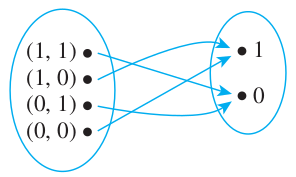
\includegraphics[scale=0.6]{../images/7.1.30.a.png}
\end{figure}
\end{proof}

\subsubsection{(b)}
\begin{center}
\arrayrulecolor{cyan}
\begin{tabular}{|ccc|c|}
\hline
\multicolumn{3}{|c|}{\cy Input} & {\cy Output} \\
\hline
$P$ & $Q$ & $R$ & $S$ \\
\hline
1 & 1 & 1 & 1 \\
\hline
1 & 1 & 0 & 0 \\
\hline
1 & 0 & 1 & 1 \\
\hline
1 & 0 & 0 & 1 \\
\hline
0 & 1 & 1 & 0 \\
\hline
0 & 1 & 0 & 0 \\
\hline
0 & 0 & 1 & 0 \\
\hline
0 & 0 & 0 & 1 \\
\hline
\end{tabular}
\arrayrulecolor{black}
\end{center}

\begin{proof}
\begin{figure}[ht!]
\centering
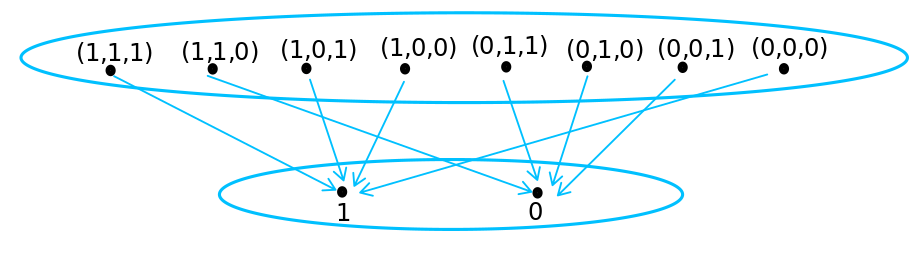
\includegraphics[scale=0.4]{../images/7.1.30.b.png}
\end{figure}
\end{proof}

\subsection{Exercise 31}
Fill in the following table to show the values of all possible two-place Boolean functions.

\begin{proof}
\begin{center}
\arrayrulecolor{cyan}
\begin{tabular}{|c|c|c|c|c|c|c|c|c|c|c|c|c|c|c|c|c|}
\hline
{\bf Input} & \(\bm{f_{1}}\) & \(\bm{f_{2}}\) & 
\(\bm{f_{3}}\) & \(\bm{f_{4}}\) & \(\bm{f_{5}}\) & 
\(\bm{f_{6}}\) & \(\bm{f_{7}}\) & \(\bm{f_{8}}\) & 
\(\bm{f_{9}}\) & \(\bm{f_{10}}\) & \(\bm{f_{11}}\) & 
\(\bm{f_{12}}\) & \(\bm{f_{13}}\) & \(\bm{f_{14}}\) & 
\(\bm{f_{15}}\) & \(\bm{f_{16}}\) \\
\hline
1 1 &0&0&0&0&0&0&0&0&1&1&1&1&1&1&1&1 \\
\hline
1 0 &0&0&0&0&1&1&1&1&0&0&0&0&1&1&1&1 \\
\hline
0 1 &0&0&1&1&0&0&1&1&0&0&1&1&0&0&1&1 \\
\hline
0 0 &0&1&0&1&0&1&0&1&0&1&0&1&0&1&0&1 \\
\hline
\end{tabular}
\arrayrulecolor{black} % change it back!
\end{center}
\end{proof}

\subsection{Exercise 32}
Consider the three-place Boolean function $f$ defined by the following rule: For each triple \((x_1, x_2, x_3)\) of
0’s and 1’s,
\[
f(x_1, x_2, x_3) = (4x_1 + 3x_2 + 2x_3) \mod 2.
\]
\subsubsection{(a)}
Find $f(1, 1, 1)$ and $f(0, 0, 1)$.

\begin{proof}
\(f(1, 1, 1) = (4 \cdot 1 + 3 \cdot 1 + 2 \cdot 1) \mod 2 = 9 \mod 2 = 1\)

\(f(0, 0, 1) = (4 \cdot 0 + 3 \cdot 0 + 2 \cdot 1) \mod 2 = 2 \mod 2 = 0\)
\end{proof}

\subsubsection{(b)}
Describe $f$ using an input/output table.

\begin{proof}
\begin{center}
\arrayrulecolor{cyan}
\begin{tabular}{|ccc|c|}
\hline
\multicolumn{3}{|c|}{\cy Input} & {\cy Output} \\
\hline
$x_1$ & $x_2$ & $x_3$ & $f(x_1, x_2, x_3)$ \\
\hline
1 & 1 & 1 & 1 \\
\hline
1 & 1 & 0 & 1 \\
\hline
1 & 0 & 1 & 0 \\
\hline
1 & 0 & 0 & 0 \\
\hline
0 & 1 & 1 & 1 \\
\hline
0 & 1 & 0 & 1 \\
\hline
0 & 0 & 1 & 0 \\
\hline
0 & 0 & 0 & 0 \\
\hline
\end{tabular}
\arrayrulecolor{black}
\end{center}
\end{proof}

\subsection{Exercise 33}
Student $A$ tries to define a function \(g: \Q \to \Z\) by
the rule
\[
g \left(\frac{m}{n}\right) = m-n \text{ for all integers } m \text{ and } n \text{ with } n \neq 0.
\]
Student $B$ claims that $g$ is not well defined. Justify student $B$'s claim.

\begin{proof}
If $g$ were well defined, then \(g(1/2) = g(2/4)\) because \(1/2 = 2/4\). However, \(g(1/2) = 1 - 2 = -1\) and 
\(g(2/4) = 2 - 4 = -2\). Since \(-1 \neq -2, g(1/2) \neq g(2/4)\). Thus $g$ is not well defined.
\end{proof}

\subsection{Exercise 34}
Student $C$ tries to define a function \(h: \Q \to \Q\) by
the rule
\[
h \left(\frac{m}{n}\right) = \frac{m^2}{n} \text{ for all integers } m \text{ and } n \text{ with } n \neq 0.
\]
Student $D$ claims that $h$ is not well defined. Justify student $D$'s claim.

\begin{proof}
\[
h(2) = h\left(\frac{4}{2}\right) = \frac{4^2}{2} = 8 \neq 4 = \frac{2^2}{1} = h\left(\frac{2}{1}\right) = h(2).
\]
\end{proof}

\subsection{Exercise 35}
Let \(U = \{1, 2, 3, 4\}\). Student $A$ tries to define a function \(R: U \to \Z\) as follows: For each \(x \in U\), 
\(R(x)\) is the integer $y$ so that \((xy) \mod 5 = 1\). Student $B$ claims that $R$ is not well defined. Who is 
right: student $A$ or student $B$? Justify your answer.

\begin{proof}
Student $B$ is correct. If $R$ were well defined, then $R(3)$ would have a uniquely determined value. However, on 
the one hand, \(R(3) = 2\) because \((3 \cdot 2) \mod 5 = 1\), and, on the other hand, \(R(3) = 7\) because 
\((3 \cdot 7) \mod 5 = 1\). Hence \(R(3)\) does not have a uniquely determined value, and so $R$ is not well defined.
\end{proof}

\subsection{Exercise 36}
Let \(V = \{1, 2, 3\}\). Student $C$ tries to define a function \(S: V \to V\) as follows: For each \(x \in V\), 
\(S(x)\) is the integer $y$ in $V$ so that \((xy) \mod 4 = 1\). Student $D$ claims that $S$ is not well defined. Who 
is right: student $C$ or student $D$? Justify your answer.

\begin{proof}
Student $D$ is right, because $S(2)$ is not defined. \(2 \cdot 1 \mod 4 = 2, 2 \cdot 2 \mod 4 = 0\), and
\(2 \cdot 3 \mod 4 = 2\). So when $x = 2$ there is no $y$ in $V$ such that \(xy \mod 4 = 1\).
\end{proof}

\subsection{Exercise 37}
On certain computers the integer data type goes from -2,147,483,648 to 2,147,483,647. Let $S$ be the set of 
all integers from -2,147,483,648 through 2,147,483,647. Try to define a function \(f: S \to S\) by the rule 
\(f(n) = n^2\) for each $n$ in $S$. Is $f$ well defined? Explain.

\begin{proof}
No, \(2,147,483,647 = 2^{31} - 1\) so for values of $n$ greater than, say, $2^{16}$, \(f(n) = n^2\) will be greater 
than $2^{32}$ which falls outside of $S$. 

Computers handle this by using 2's complement and looping the overshoot around back to \(-2^{31}\) and onward toward 
the positive values again. Here is an example from Scala:

\begin{minted}{scala}
$ scala
// Welcome to Scala 3.3.0 (17.0.7, Java OpenJDK 64-Bit Server VM). 
// Type in expressions for evaluation. Or try :help.
scala> def f(n: Int): Int = n*n
def f(n: Int): Int                                    
scala> f(2147483647)
val res0: Int = 1
scala> 
\end{minted}
\end{proof}

\subsection{Exercise 38}
Let \(X = \{a,b,c\}\) and \(Y = \{r,s,t,u,v,w\}\). Define \(f: X \to Y\) as follows: \(f(a) = b, f(b) = v, f(c) = t\).

\subsubsection{(a)}
Draw an arrow diagram for $f$.

\begin{proof}
\begin{figure}[ht!]
\centering
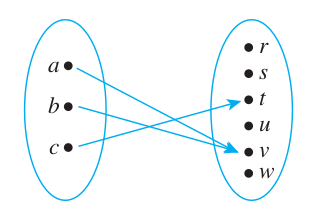
\includegraphics[scale=0.5]{../images/7.1.38.a.png}
\end{figure}
\end{proof}

\subsubsection{(b)}
Let \(A = \{a, b\}, C = \{t\}, D = \{u, v\}, E = \{r, s\}\). 

Find \(f(A), f(X), f^{-1}(C), f^{-1}(D), f^{-1}(E), f^{-1}(Y)\).

\begin{proof}
\(f(A) = \{v\}, f(X) = \{t, v\}, f^{-1}(C) = \{c\}, f^{-1}(D) = \{a, b\}, f^{-1}(E) = \es\), 

\(f^{-1}(Y) = \{a,b,c\}\)
\end{proof}

\subsection{Exercise 39}
Let \(X = \{1, 2, 3, 4\}\) and \(Y = \{a, b, c, d, e\}\). Define \(g: X \to Y\) as follows: 
\(g(1) = a, g(2) = a, g(3) = a, g(4) = d\).

\subsubsection{(a)}
Draw an arrow diagram for $g$.

\begin{proof}
\begin{figure}[ht!]
\centering
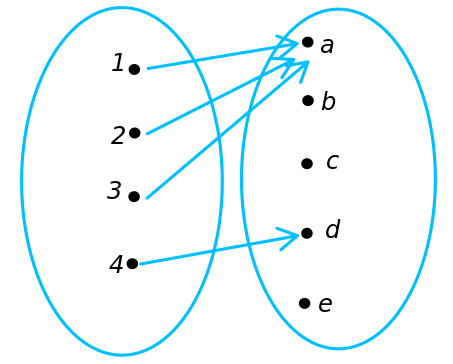
\includegraphics[scale=0.3]{../images/7.1.39.a.png}
\end{figure}
\end{proof}

\subsubsection{(b)}
Let \(A = \{2, 3\}, C = \{a\}\), and \(D = \{b, c\}\). Find \(g(A), g(X), g^{-1}(C), g^{-1}(D)\), and \(g^{-1}(Y)\).

\begin{proof}
\(g(A) = \{a\}, g(X) = \{a, d\}, g^{-1}(C) = \{1, 2, 3\}, g^{-1}(D) = \es, g^{-1}(Y) = \{1, 2, 3, 4\}\).
\end{proof}

\subsection{Exercise 40}
Let $X$ and $Y$ be sets, let $A$ and $B$ be any subsets of $X$, and let $F$ be a function from $X$ to $Y$. Fill in the 
blanks in the following proof that \(F(A) \cup F (B) \subseteq F(A \cup B)\).

{\bf Proof:} Let $y$ be any element in \(F(A) \cup F(B)\). {\it [We must show that $y$ is in \(F(A \cup B)\).]} By 
definition of union, {\cy (i) \fbl.} 

{\bf Case 1, \(\bm{y \in F(A)}\):} In this case, by definition of $F(A)$, \(y = F(x)\) for {\cy (ii) \fbl} 
\(x \in A\). Since \(A \subseteq A \cup B\), it follows from the definition of union that \(x \in\) {\cy (iii) 
\fbl.} Hence, \(y = F(x)\) for some \(x \in A \cup B\), and thus, by definition of \(F(A \cup B), y \in\) {\cy (iv) \fbl.}

{\bf Case 2, \(\bm{y \in F(B)}\):} In this case, by definition of $F(B)$, {\cy (v) \fbl} for some $x \in B$. 
Since \(B \subseteq A \cup B\) it follows from the definition of union that {\cy (vi) \fbl.} 
Thus \(y \in F(A \cup B)\).

Therefore, regardless of whether \(y \in F(A)\) or \(y \in F(B)\), we have that \(y \in F(A \cup B)\) {\it [as was to be shown].}

\begin{proof}
(i) \(y \in F(A)\) or \(y \in F(B)\) (ii) some (iii) \(A \cup B\) (iv) \(F(A \cup B)\) (v) \(y = F(x)\) (vi) \(x \in A \cup B\)
\end{proof}

{\bf \cy In $41-49$ let $X$ and $Y$ be sets, let $A$ and $B$ be any subsets of $X$, and let $C$ and $D$ be any 
subsets of $Y$. Determine which of the properties are true for every function $F$ from $X$ to $Y$ and which are false 
for at least one function $F$ from $X$ to $Y$. Justify your answers.}

\subsection{Exercise 41}
If \(A \subseteq B\) then \(F(A) \subseteq F(B)\).

\begin{proof}
Let $F$ be a function from $X$ to $Y$, and suppose \(A \subseteq X, B \subseteq X\), and \(A \subseteq B\). 
Let \(y \in F(A)\). {\it [We must show that \(y \in F(B)\).]} By definition of image of a set, \(y = F(x)\) for 
some \(x \in A\). Thus since \(A \subseteq B, x \in B\), and so \(y = F(x)\) for some \(x \in B\). 
Hence \(y \in F(B)\) {\it [as was to be shown].}
\end{proof}

\subsection{Exercise 42}
\(F(A \cap B) \subseteq F(A) \cap F(B)\)

\begin{proof}
1. Assume \(y \in F(A \cap B)\). {\it [We want to show \(y \in F(A) \cap F(B)\).]} 

2. By 1 and definition of \(F(A \cap B)\), \(y = F(x)\) for some \(x \in A \cap B\).

3. By 2 and definition of intersection, \(x \in A\) and \(x \in B\).

4. By 3 and definition of $F(A)$ and $F(B)$, \(y = F(x)\) is in $F(A)$ and in $F(B)$.

5. By 4 and definition of intersection, \(y \in F(A) \cap F(B)\).

6. By 1, 5 and definition of subset, \(F(A \cap B) \subseteq F(A) \cap F(B)\).
\end{proof}

\subsection{Exercise 43}
\(F(A) \cap F(B) \subseteq F(A \cap B)\)

\begin{proof}
\begin{figure}[ht!]
\centering
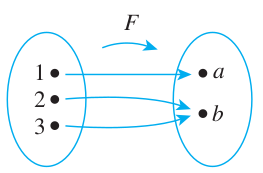
\includegraphics[scale=0.5]{../images/7.1.43.png}
\end{figure}
\underline{Counterexample:} Let \(X = \{1, 2, 3\}\), let \(Y = \{a, b\}\), and define a function \(F: X \to Y\) 
by the arrow diagram shown above.

Let \(A = \{1, 2\}\) and \(B = \{1, 3\}\). Then \(F(A) = \{a, b\} = F(B)\), and so \(F(A) \cap F(B) = \{a, b\}\). But 
\(F(A \cap B) = F(\{1\}) = \{a\} \neq \{a, b\}\). And so \(F(A) \cap F(B) \nsubseteq F(A \cap B)\). (This is just one 
of many possible counterexamples.)
\end{proof}

\subsection{Exercise 44}
For all subsets $A$ and $B$ of $X$, \(F(A - B) = F(A) - F(B)\).

\begin{proof}
\underline{Counterexample:} Let \(X = \{1, 2\}, Y = \{a\}, A = \{1\}, B = \{2\}\), define \(F: X \to Y\) by 
\(F(1) = F(2) = a\). Then \(A - B = \{1\}, F(A) = \{a\}, F(B)=\{a\}\). So \(F(A-B) = \{a\} \neq \es = F(A) - F(B)\).
\end{proof}

\subsection{Exercise 45}
For all subsets $C$ and $D$ of $Y$, if \(C \subseteq D\) then \(F^{-1}(C) \subseteq F^{-1}(D)\).

\begin{proof}
Let $F$ be a function from a set $X$ to a set $Y$, and suppose \(C \subseteq Y, D \subseteq Y\), and 
\(C \subseteq D\). {\it [We must show that \(F^{-1}(C) \subseteq F^{-1}(D)\).]} Suppose \(x \in F^{-1}(C)\). Then 
\(F(x) \in C\). Since \(C \subseteq D, F(x) \in D\) also. Hence, by definition of inverse image, \(x \in F^{-1}(D)\). 
{\it [So \(F^{-1}(C) \subseteq F^{-1}(D)\).]}
\end{proof}

\subsection{Exercise 46}
For all subsets $C$ and $D$ of $Y$, \(F^{-1}(C \cup D) = F^{-1}(C) \cup F^{-1}(D)\).

\begin{proof}
1. Assume \(x \in F^{-1}(C \cup D)\) and let $y = F(x)$. {\it [Want to show \(x \in F^{-1}(C) \cup F^{-1}(D)\).]}

2. By 1 and definition of \(F^{-1}(C \cup D)\), \(y \in C \cup D\).

3. By 2 and definition of union, \(y \in C\) or \(y \in D\).

4. {\bf Case 1 (\(\bm{y \in C}\)):} By definition of \(F^{-1}(C)\), \(x \in F^{-1}(C)\). 

By definition of union, \(x \in F^{-1}(C) \cup F^{-1}(D)\).

5. {\bf Case 2 (\(\bm{y \in D}\)):} By definition of \(F^{-1}(D)\), \(x \in F^{-1}(D)\). 

By definition of union, \(x \in F^{-1}(C) \cup F^{-1}(D)\).

6. By 4 and 5, \(x \in F^{-1}(C) \cup F^{-1}(D)\).

7. By 1, 6 and definition of subset, \(F^{-1}(C \cup D) \subseteq F^{-1}(C) \cup F^{-1}(D)\).

The proof of the reverse direction \(F^{-1}(C) \cup F^{-1}(D) \subseteq F^{-1}(C \cup D)\) is similar.
\end{proof}

\subsection{Exercise 47}
For all subsets $C$ and $D$ of $Y$, \(F^{-1}(C \cap D) = F^{-1}(C) \cap F^{-1}(D)\).

\begin{proof}
True, the proof is extremely similar to exercise 46.
\end{proof}

\subsection{Exercise 48}
For all subsets $C$ and $D$ of $Y$, \(F^{-1}(C-D) = F^{-1}(C) - F^{-1}(D)\).

\begin{proof}
1. Assume \(x \in F^{-1}(C-D)\) and let $y = F(x)$. {\it [Want to show \(x \in F^{-1}(C) - F^{-1}(D)\).]}

2. By 1 and definition of \(F^{-1}(C-D), y \in C-D\).

3. By 2 and definition of difference, \(y \in C\) and \(y \notin D\).

4. By 3 and definition of \(F^{-1}(C)\), \(x \in F^{-1}(C)\). Similarly, since $y = F(x)$ and $y \notin D$, 
\(x \notin F^{-1}(D)\).

5. By 4 and definition of difference, \(x \in F^{-1}(C) - F^{-1}(D)\).

6. By 1, 5 and definition of subset, \(F^{-1}(C-D) \subseteq F^{-1}(C) - F^{-1}(D)\).

{\it Now the reverse part:}

7. Assume \(x \in F^{-1}(C) - F^{-1}(D)\) and let $y = F(x)$. {\it [Want to show \(x \in F^{-1}(C-D)\).]}

8. By 7 and definition of difference, \(x \in F^{-1}(C)\) and \(x \notin F^{-1}(D)\).

9. By 8 and definition of \(F^{-1}(C), y \in C\). Similarly \(y \notin D\).

10. By 9 and definition of difference \(y \in C-D\).

11. Since $y = F(x)$, by 10 and definition of \(F^{-1}(C-D)\), \(x \in F^{-1}(C-D)\).

12. By 7, 11 and definition of subset, \(F^{-1}(C) - F^{-1}(D) \subseteq F^{-1}(C-D)\).

{\it Conclusion:}

13. By 6, 12 and definition of set equality \(F^{-1}(C) - F^{-1}(D) = F^{-1}(C-D)\).
\end{proof}

\subsection{Exercise 49}
\(F(F^{-1}(C)) \subseteq C\).

\begin{proof}
1. Assume \(y \in F(F^{-1}(C))\). {\it [Want to show \(y \in C\).]}

2. By 1 and definition of \(F(F^{-1}(C))\), there exists some \(x \in F^{-1}(C)\) such that \(y = F(x)\).

3. By 2 and definition of \(F^{-1}(C)\), \(F(x) \in C\). So $y \in C$ because $y = F(x)$.

4. By 1, 3 and definition of subset, \(F(F^{-1}(C)) \subseteq C\).
\end{proof}

\subsection{Exercise 50}
Given a set $S$ and a subset $A$, the characteristic function of $A$, denoted $\chi_A$, is the function defined 
from $S$ to $\Z$ with the property that for each $u \in S$,
\[
\chi_A(u) =
\left\{
\begin{tabular}{lr}
\(1\) & if \(u \in A\) \\
\(0\) & if \(u \notin A\)
\end{tabular}
\right.
\]
Show that each of the following holds for all subsets $A$ and $B$ of $S$ and every $u \in S$.

\subsubsection{(a)}
\(\chi_{A \cap B}(u) = \chi_A(u) \cdot \chi_B(u)\)

\begin{proof}
Assume $A, B$ are any subsets of $S$ and $u$ is any element in $S$. There are 4 cases:

{\bf Case 1 (\(\bm{u \in A, u \in B}\)):} Then \(\chi_A(u) = 1 \) and \(\chi_B(u) = 1\). 

By definition of intersection \(u \in A \cap B\). Thus
\(\chi_{A \cap B}(u) = 1\) also. Since $1 = 1 \cdot 1$,
\(\chi_{A \cap B}(u) = \chi_A(u) \cdot \chi_B(u)\).

{\bf Case 2 (\(\bm{u \in A, u \notin B}\)):} Then \(\chi_A(u) = 1 \) and \(\chi_B(u) = 0\). 

By definition of intersection \(u \notin A \cap B\). Thus
\(\chi_{A \cap B}(u) = 0\) also. Since $0 = 1 \cdot 0$,
\(\chi_{A \cap B}(u) = \chi_A(u) \cdot \chi_B(u)\).

{\bf Case 3 (\(\bm{u \notin A, u \in B}\)):} Then \(\chi_A(u) = 0 \) and \(\chi_B(u) = 1\). 

By definition of intersection \(u \notin A \cap B\). Thus
\(\chi_{A \cap B}(u) = 0\) also. Since $0 = 0 \cdot 1$,
\(\chi_{A \cap B}(u) = \chi_A(u) \cdot \chi_B(u)\).

{\bf Case 4 (\(\bm{u \notin A, u \notin B}\)):} Then \(\chi_A(u) = 0 \) and \(\chi_B(u) = 0\). 

By definition of intersection \(u \notin A \cap B\). Thus
\(\chi_{A \cap B}(u) = 0\) also. Since $0 = 0 \cdot 0$,
\(\chi_{A \cap B}(u) = \chi_A(u) \cdot \chi_B(u)\).
\end{proof}

\subsubsection{(b)}
\(\chi_{A \cup B}(u) = \chi_A(u) + \chi_B(u) - \chi_A(u) \cdot \chi_B(u)\)

\begin{proof}
Assume $A, B$ are any subsets of $S$ and $u$ is any element in $S$. There are 4 cases:

{\bf Case 1 (\(\bm{u \in A, u \in B}\)):} Then \(\chi_A(u) = 1 \) and \(\chi_B(u) = 1\). 

By definition of union \(u \in A \cup B\). Thus
\(\chi_{A \cup B}(u) = 1\) also. 
Since $1 = 1 + 1 - (1 \cdot 1)$, \(\chi_{A \cup B}(u) = \chi_A(u) + \chi_B(u) - \chi_A(u) \cdot \chi_B(u)\).

{\bf Case 2 (\(\bm{u \in A, u \notin B}\)):} Then \(\chi_A(u) = 1\) and \(\chi_B(u) = 0\). 

By definition of union \(u \in A \cup B\). Thus
\(\chi_{A \cup B}(u) = 1\) also. 
Since $1 = 1 + 0 - (1 \cdot 0)$, \(\chi_{A \cup B}(u) = \chi_A(u) + \chi_B(u) - \chi_A(u) \cdot \chi_B(u)\).

{\bf Case 3 (\(\bm{u \notin A, u \in B}\)):} Then \(\chi_A(u) = 0\) and \(\chi_B(u) = 1\). 

By definition of union \(u \in A \cup B\). Thus
\(\chi_{A \cup B}(u) = 1\) also. 
Since $1 = 0 + 1 - (0 \cdot 1)$, \(\chi_{A \cup B}(u) = \chi_A(u) + \chi_B(u) - \chi_A(u) \cdot \chi_B(u)\).

{\bf Case 4 (\(\bm{u \notin A, u \notin B}\)):} Then \(\chi_A(u) = 0 \) and \(\chi_B(u) = 0\). 

By definition of union \(u \notin A \cup B\). Thus
\(\chi_{A \cup B}(u) = 0\) also. 
Since $0 = 0 + 0 - (0 \cdot 0)$, \(\chi_{A \cup B}(u) = \chi_A(u) + \chi_B(u) - \chi_A(u) \cdot \chi_B(u)\).
\end{proof}

{\bf \cy Each of exercises $51-53$ refers to the Euler phi function, denoted $\phi$, which is defined as follows: For 
each integer \(n \geq 1\), $\phi(n)$ is the number of positive integers less than or equal to $n$ that have no 
common factors with $n$ except $\pm 1$. For example, \(\phi(10) = 4\) because there are four positive integers 
less than or equal to 10 that have no common factors with 10 except $\pm 1$, namely, 1, 3, 7, and 9.}

\subsection{Exercise 51}
Find each of the following:

\subsubsection{(a)}
\(\phi(15)\)

\begin{proof}
\(\phi(15) = 8\) {\it [because $1, 2, 4, 7, 8, 11, 13$, and $14$ have no common factors with $15$ other than $\pm 1$]}
\end{proof}

\subsubsection{(b)}
\(\phi(2)\)

\begin{proof}
\(\phi(2) = 1\) {\it [because the only positive integer less than or equal to $2$ having no common factors with $2$ 
other than $\pm 1$ is $1$]}
\end{proof}

\subsubsection{(c)}
\(\phi(5)\)

\begin{proof}
\(\phi(5) = 4\) {\it [because $1, 2, 3$, and $4$ have no common factors with $5$ other than $\pm 1$]}
\end{proof}

\subsubsection{(d)}
\(\phi(12)\)

\begin{proof}
\(\phi(12) = 4\) (1, 5, 7, 11)
\end{proof}

\subsubsection{(e)}
\(\phi(11)\)

\begin{proof}
\(\phi(11) = 10\) (1, 2, 3, 4, 5, 6, 7, 8, 9, 10)
\end{proof}

\subsubsection{(f)}
\(\phi(1)\)

\begin{proof}
\(\phi(1) = 1\)
\end{proof}

\subsection{Exercise 52}
Prove that if $p$ is a prime number and $n$ is an integer with \(n \geq 1\), then \(\phi(p^n) = p^n - p^{n-1}\).

\begin{proof}
Let $p$ be any prime number and $n$ any integer with \(n \geq 1\). There are \(p^{n-1}\) positive integers less than 
or equal to \(p^n\) that have a common factor other than $\pm 1$ with \(p^n\), namely, \(p, 2p, 3p, \ldots, 
(p^{n-1})p\). Hence, there are \(p^n - p^{n-1}\) positive integers less than or equal to \(p^n\) that do not have a 
common factor with \(p^n\) except for $\pm 1$.
\end{proof}

\subsection{Exercise 53}
Prove that there are infinitely many integers $n$ for which \(\phi(n)\) is a perfect square.

\begin{proof}
By exercise 52, for any integer $n$ with \(n \geq 1, \phi(2^n) = 2^n - 2^{n-1} = 2^{n-1}\).

So, for all integers $k$ with $k \geq 1$, we have that \(\phi(2^{2k+1}) = 2^{2k} = (2^k)^2\) is a perfect square.
\end{proof}

\section{Exercise Set 7.2}

\subsection{Exercise 1}
The definition of one-to-one is stated in two ways:
\[
\forall x_1, x_2 \in X, \text{ if } F(x_1) = F(x_2) \text{ then } x_1 = x_2
\]
and 
\[
\forall x_1, x_2 \in X, \text{ if } x_1 \neq x_2 \text{ then } F(x_1) \neq F(x_2).
\]
Why are these two statements logically equivalent?

\begin{proof}
The second statement is the contrapositive of the first.
\end{proof}

\subsection{Exercise 2}
Fill in each blank with the word most or least.

\subsubsection{(a)}
A function $F$ is one-to-one if, and only if, each element in the co-domain of $F$ is the image of at \fbl one element 
in the domain of $F$.

\begin{proof}
most
\end{proof}

\subsubsection{(b)}
A function $F$ is onto if, and only if, each element in the co-domain of $F$ is the image of at \fbl one element in the 
domain of $F$.

\begin{proof}
least
\end{proof}

\subsection{Exercise 3}
When asked to state the definition of one-to-one, a student replies, “A function $f$ is one-to-one if, and only if, 
every element of $X$ is sent by $f$ to exactly one element of $Y$.” Give a counterexample to show that the student’s 
reply is incorrect.

\begin{proof}
One counterexample is given and explained below. Give a different counterexample and accompany it with an explanation. 

\underline{Counterexample:} Consider \(X = \{a,b\}, Y = \{u,v\}\) and the function $f$ defined by\(f(a) = f(b) =u\).
Observe that $a$ is sent to exactly one element of $Y$, namely, $u$, and $b$ is also sent to exactly one element of 
$Y$, namely, $u$ also. So it is true that every element of $X$ is sent to exactly one element of $Y$. But $f$ is not 
one-to-one because $f(a) = f(b)$ whereas $a \neq b$. {\it [Note that to say, “Every element of $X$ is sent to exactly 
one element of $Y$” is just another way of saying that in the arrow diagram for the function there is only one arrow 
coming out of each element of $X$. But this statement is part of the definition of any function, not just of a 
one-to-one function.]}
\end{proof}

\subsection{Exercise 4}
Let \(f: X \to Y\) be a function. True or false? A sufficient condition for $f$ to be one-to-one is that for
every element $y$ in $Y$, there is at most one $x$ in $X$
with \(f(x) = y\). Explain your answer.

\begin{proof}
True. Assume \(x_1, x_2 \in X\) and assume \(f(x_1) = f(x_2)\). {\it [We want to show \(x_1 = x_2\)].} Let 
\(y = f(x_1) = f(x_2)\). By assumption there is at most one $x$ in $X$ such that $y = f(x)$. Thus \(x = x_1 = x_2\),
{\it [as was to be shown.]}
\end{proof}

\subsection{Exercise 5}
All but two of the following statements are correct ways to express the fact that a function $f$ is onto. 
Find the two that are incorrect.

\subsubsection{(a)}
$f$ is onto $\iff$ every element in its co-domain is the image of some element in its domain.

\begin{proof}
Correct.
\end{proof}

\subsubsection{(b)}
$f$ is onto $\iff$ every element in its domain has a corresponding image in its co-domain.

\begin{proof}
Incorrect.
\end{proof}

\subsubsection{(c)}
$f$ is onto \(\iff  \forall y \in Y, \exists x \in X\) such that \(f(x) = y\).

\begin{proof}
Correct.
\end{proof}

\subsubsection{(d)}
$f$ is onto \(\iff \forall x \in X, \exists y \in Y\) such that \(f(x) = y\).

\begin{proof}
Incorrect.
\end{proof}

\subsubsection{(e)}
$f$ is onto $\iff$ the range of $f$ is the same as the co-domain of $f$.

\begin{proof}
Correct.
\end{proof}

\subsection{Exercise 6}
Let \(X = \{1, 5, 9\}, Y = \{3, 4, 7\}\).

\subsubsection{(a)}
Define \(f: X \to Y\) by specifying that \(f(1) = 4, f(5) = 7, f(9) = 4\). Is $f$ one-to-one? Is $f$ onto? 
Explain your answers.

\begin{proof}
Not 1-1: \(f(1) = f(9)\) but \(1 \neq 9\). Not onto: no $x \in X$ such that $f(x) = 3$.
\end{proof}

\subsubsection{(b)}
Define \(g: X \to Y\) by specifying that \(g(1) = 7, g(5) = 3, g(9) = 4\). Is $g$ one-to-one? Is $g$ onto? 
Explain your answers.

\begin{proof}
$g$ is 1-1, because \(g(1) \neq f(5), g(1) \neq g(9)\) and \(g(1) \neq g(9)\).

$g$ is onto because each element of $Y$ is the image of some $x \in X$: \(3 = g(5), 4 = g(9), 7 = g(1)\).
\end{proof}

\subsection{Exercise 7}
Let \(X = \{a, b, c, d\}\) and \(Y = \{e, f, g\}\). Define
functions $F$ and $G$ by the arrow diagrams below.

\begin{figure}[ht!]
\centering
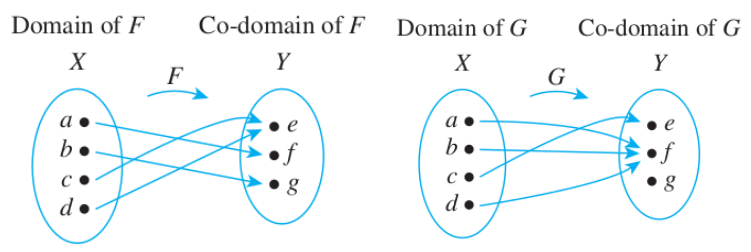
\includegraphics[scale=0.5]{../images/7.2.7.png}
\end{figure}

\subsubsection{(a)}
Is $F$ one-to-one? Why or why not? Is it onto? Why or why not?

\begin{proof}
$F$ is not 1-1 because $F(c) = F(d)$ but $c \neq d$.

$F$ is onto, because each element in $Y$ is the image of some element in $X$.
\end{proof}

\subsubsection{(b)}
Is $G$ one-to-one? Why or why not? Is it onto? Why or why not?

\begin{proof}
$G$ is 1-1 because $G(a) \neq G(b), G(a) \neq G(c)$ and $G(b) \neq G(c)$.

$G$ is not onto, because there is no $x \in X$ such that $G(x) = g$.
\end{proof}

\subsection{Exercise 8}
Let \(X = \{a, b, c\}\) and \(Y = \{d, e, f, g\}\). Define
functions $H$ and $K$ by the arrow diagrams below.

\begin{figure}[ht!]
\centering
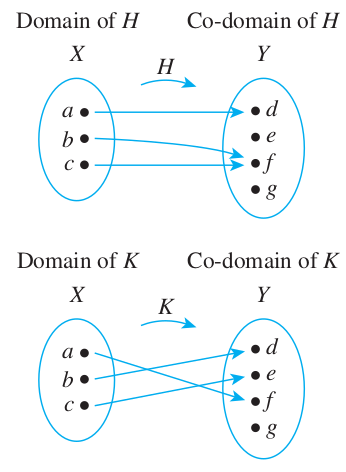
\includegraphics[scale=0.5]{../images/7.2.8.png}
\end{figure}

\subsubsection{(a)}
Is $H$ one-to-one? Why or why not? Is it onto? Why or why not?

\begin{proof}
$H$ is not 1-1 because \(H(b) = H(c)\) but \(b \neq c\).

$H$ is not onto, because there is no $x \in X$ such that $H(x) = g$.
\end{proof}

\subsubsection{(b)}
Is $K$ one-to-one? Why or why not? Is it onto? Why or why not?

\begin{proof}
$K$ is 1-1 because \(K(a) \neq K(b), K(a) \neq K(c)\) and \(K(b) \neq K(c)\).

$K$ is not onto, because there is no $x \in X$ such that $K(x) = g$.
\end{proof}

\subsection{Exercise 9}
Let \(X = \{1, 2, 3\}, Y = \{1, 2, 3, 4\}\), and \(Z = \{1, 2\}\).

\subsubsection{(a)}
Define a function \(f: X \to Y\) that is one-to-one but not onto.

\begin{proof}
One example of many is the following:
\begin{figure}[ht!]
\centering
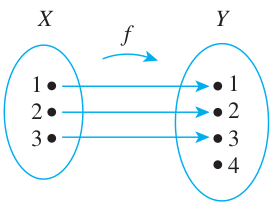
\includegraphics[scale=0.5]{../images/7.2.9.png}
\end{figure}
\end{proof}

\subsubsection{(b)}
Define a function \(g: X \to Z\) that is onto but not one-to-one.

\begin{proof}
Let \(g(1) = 1, g(2) = 2, g(3) = 2\).
\end{proof}

\subsubsection{(c)}
Define a function \(h: X \to X\) that is neither one-to-one nor onto.

\begin{proof}
Let \(h(1) = 1, h(2) = 1, h(3) = 1, h(4) = 1\).
\end{proof}

\subsubsection{(d)}
Define a function \(k: X \to X\) that is one-to-one and onto but is not the identity function on $X$.

\begin{proof}
Let \(k(1) = 2, k(2) = 3, k(3) = 4, k(4) = 1\).
\end{proof}

\subsection{Exercise 10}
\subsubsection{(a)}
Define \(f: \Z \to \Z\) by the rule \(f(n) = 2n\), for every integer $n$.

(i) Is $f$ one-to-one? Prove or give a counterexample.

(ii) Is $f$ onto? Prove or give a counterexample.

\begin{proof}
(i) $f$ is one-to-one. Suppose \(f(n_1) = f(n_2)\) for some integers $n_1$ and $n_2$. {\it [We must show that \(n_1 = 
n_2\).]} By definition of \(f, 2n_1 = 2n_2\), and dividing both sides by 2 gives $n_1 = n_2$ {\it [as was to be shown].}

(ii) $f$ is not onto. \underline{Counterexample:} Consider \(1 \in \Z\). We claim that \(1 \neq f(n)\), for any 
integer $n$, because if there were an integer $n$ such that \(1 = f(n)\), then, by definition of \(f, 1 = 2n\). 
Dividing both sides by 2 would give \(n = 1/2\). But $1/2$ is not an integer. Hence \(1 \neq f(n)\) for any integer 
$n$, and so $f$ is not onto.
\end{proof}

\subsubsection{(b)}
Let $2\Z$ denote the set of all even integers. That is, 
\[
2\Z = \{n \in \Z \,|\,n=2k, \text{ for some integer } k\}.
\]
Define \(h: \Z \to 2\Z\) by the rule \(h(n) = 2n\), for each integer $n$. Is $h$ onto? Prove or give a counterexample.

\begin{proof}
$h$ is onto. Suppose \(m \in 2\Z\). {\it [We must show that there exists an integer such that $h$ of that integer 
equals $m$.]} Since \(m \in 2\Z, m = 2k\) for some integer $k$. Then \(h(k) = 2k = m\). Hence there exists an integer 
(namely, $k$) such that \(h(k) = m\) {\it [as to be shown].}
\end{proof}

\subsection{Exercise 11}
\subsubsection{(a)}
Define \(g: \Z \to \Z\) by the rule \(g(n) = 4n - 5\), for every integer $n$.

(i) Is $g$ one-to-one? Prove or give a counterexample.

(ii) Is $g$ onto? Prove or give a counterexample.

\begin{proof}
$g$ is 1-1: assume \(n_1, n_2 \in \Z\) and \(g(n_1) = g(n_2)\). {\it [We want to show \(n_1 = n_2\)].} By $g$'s
definition \(4n_1-5=4n_2-5\). Adding 5 to both sides and dividing both sides by 4 we get \(n_1 = n_2\).

$g$ is not onto: there is no $n \in \Z$ such that $g(n) = 0$. Argue by contradiction and assume \(g(n) = 0\) for some
\(n \in \Z\). Then \(4n-5 = 0\) so \(n = 5/4\) which is not an integer, a contradiction.
\end{proof}

\subsubsection{(b)}
Define \(G: \R \to \R\) by the rule \(G(x) = 4x - 5\), for every real number $x$. Is $G$ onto? Prove or give a counterexample.

\begin{proof}
$G$ is onto. Suppose $y$ is any element of $\R$. {\it [We must show that there is an element $x$ in $\R$ such that 
\(G(x) = y\). What would $x$ be if it exists? Scratch work shows that $x$ would have to equal \((y + 5)/4\). The proof 
must then show that $x$ has the necessary properties.]} Let \(x = (y + 5)/4\). Then (1) \(x \in \R\), and (2) \(G(x) = 
G((y + 5)/4) = 4[(y + 5)/4] - 5 = (y + 5) - 5 = y\) {\it [as was to be shown].}
\end{proof}

\subsection{Exercise 12}
\subsubsection{(a)}
Define \(F: \Z \to \Z\) by the rule \(F(n) = 2 - 3n\), for each integer $n$.

(i) Is $F$ one-to-one? Prove or give a counterexample.

(ii) Is $F$ onto? Prove or give a counterexample.

\begin{proof}
$F$ is 1-1: assume \(n_1, n_2 \in \Z\) and \(F(n_1) = F(n_2)\). {\it [We want to show \(n_1 = n_2\).]} By $F$'s
definition, \(2 - 3n_1 = 2-3n_2\). Subtracting 2 from both sides and dividing by $-3$ we get \(n_1 = n_2\).

$F$ is not onto: there is no \(n \in \Z\) such that \(F(n) = 0\). Because otherwise \(2 - 3n = 0\) for some integer 
$n$, but then \(n = 2/3\) which is not an integer, a contradiction.
\end{proof}

\subsubsection{(b)}
Define \(G: \R \to \R\) by the rule \(G(x) = 2 - 3x\), for each real number $x$. Is $G$ onto? Prove or give a counterexample.

\begin{proof}
$G$ is 1-1 just like $F$ above. Same proof applies.

$G$ is also onto: for every $y \in \R$ there exists an $x \in \R$ such that $G(x) = y$: let \(x = (y - 2) / (-3)\).
Then \(\dps G(x) = G((y - 2) / (-3)) = 2 - 3 \cdot \frac{y-2}{-3} = 2 + (y-2) = y\).
\end{proof}

\subsection{Exercise 13}
\subsubsection{(a)}
Define \(H: \R \to \R\) by the rule \(H(x) = x^2\), for each real number $x$.

(i) Is $H$ one-to-one? Prove or give a counterexample.

(ii) Is $H$ onto? Prove or give a counterexample.

\begin{proof}
(i) $H$ is not one-to-one. \underline{Counterexample:} \(H(1) = 1 = H(-1)\) but \(1 \neq -1\).

(ii) H is not onto. \underline{Counterexample:} \(H(x) \neq -1\) for any real number $x$ because \(H(x) = x^2\) and no 
real numbers have negative squares.
\end{proof}

\subsubsection{(b)}
Define \(K: \R^{nonneg} \to \R^{nonneg}\) by the rule \(K(x) = x^2\), for each nonnegative real number $x$. 
Is $K$ onto? Prove or give a counterexample.

\begin{proof}
$K$ is onto. Given any \(y \in \R^{nonneg}\) let \(x = \sqrt{y}\). Then \(K(x) = K(\sqrt{y}) = (\sqrt{y})^2 = y\).
\end{proof}

\subsection{Exercise 14}
Explain the mistake in the following “proof.”

{\bf Theorem:} The function \(f: \Z \to \Z\) defined by the formula \(f(n) = 4n + 3\), for each integer $n$, is one-to-one.

{\bf “Proof:} Suppose any integer $n$ is given. Then by definition of $f$, there is only one possible value for 
$f(n)$, namely, \(4n + 3\). Hence $f$ is one-to-one.”

\begin{proof}
The “proof” claims that $f$ is one-to-one because for each integer $n$ there is only one possible value for $f(n)$. 
But to say that for each integer $n$ there is only one possible value for $f(n)$ is just another way of saying 
that $f$ satisfies one of the conditions necessary for it to be a function. To show that $f$ is one-to-one, one must 
show that any integer $n$ has a different function value from that of the integer $m$ whenever \(n \neq m\).
\end{proof}

{\bf \cy In each of $15-18$ a function $f$ is defined on a set of real numbers. Determine whether or not $f$ is one-
to-one and justify your answer.}

\subsection{Exercise 15}
\(\dps f(x) = \frac{x+1}{x}\), for each real number \(x \neq 0\)

\begin{proof}
$f$ is 1-1: Suppose \(f(x_1) = f(x_2)\) where $x_1$ and $x_2$ are nonzero real numbers. {\it [We must show that 
\(x_1 = x_2\).]} By definition of $f$,
\[
\frac{x_1 + 1}{x_1} = \frac{x_2 + 1}{x_2}
\]
Cross-multiplying gives \(x_1x_2 + x_2 = x_1x_2 + x_1\) and subtracting $x_1x_2$ gives \(x_1 = x_2\).
\end{proof}

\subsection{Exercise 16}
\(\dps f(x) = \frac{x}{x^2+1}\), for each real number \(x\)

\begin{proof}
$f$ is not one-to-one. \underline{Counterexample:} Note that

\begin{center}
\begin{tabular}{ccccccc}
\(\dps\frac{x_1}{x_1^2+1}\) & = & \(\dps\frac{x_2}{x_2^2+1}\) & \(\implies\) & \(x_1x_2^2 + x_1\) & = & \(x_2x_1^2 + x_2\)\\
&&&\(\implies\) & \(x_1x_2^2 - x_2x_1^2\) & = & \(x_2-x_1\)\\
&&&\(\implies\) & \(x_1x_2(x_2-x_1)\) & = & \(x_2-x_1\)\\
&&&\(\implies\) & \(x_1 = x_2\) & or & \(x_1x_2 = 1\).
\end{tabular}
\end{center}

Thus take any $x_1$ and $x_2$ with $x_1 \neq x_2$ but $x_1x_2 = 1$. For instance, take 
\(x_1 = 2\) and \(x_2 = 1/2\). Then \(f(x_1) = f(2) = 2/5\) and \(f(x_2) = f(1/2) = 2/5\), but $2 \neq 1/2$.
\end{proof}

\subsection{Exercise 17}
\(\dps f(x) = \frac{3x-1}{x}\), for each real number \(x \neq 0\)

\begin{proof}
$f$ is 1-1: Assume \(x_1 \neq 0 \neq x_2\) and assume \(\frac{3x_1-1}{x_1} = \frac{3x_2-1}{x_2}\).
{\it [We want to show \(x_1 = x_2\).]} Cross-multiplying gives \((3x_1-1)x_2 = (3x_2-1)x_1\). So
\(3x_1x_2 - x_2 = 3x_1x_2 - x_1\). Canceling $3x_1x_2$ gives \(-x_2 = -x_1\), so \(x_1 = x_2\).
\end{proof}

\subsection{Exercise 18}
\(\dps f(x) = \frac{x+1}{x-1}\), for each real number \(x \neq 1\)

\begin{proof}
$f$ is 1-1: Assume \(x_1 \neq 1 \neq x_2\) and assume \(\frac{x_1+1}{x_1-1} = \frac{x_2+1}{x_2-1}\).
{\it [We want to show \(x_1 = x_2\).]} Cross-multiplying gives \((x_1+1)(x_2-1) = (x_2+1)(x_1-1)\). So
\(x_1x_2 - x_1 + x_2 - 1 = x_1x_2 + x_1 - x_2 - 1\). Canceling $x_1x_2 - 1$ gives \(-x_1 + x_2 = x_1 - x_2\), so 
\(2x_2 = 2x_1\) and dividing by 2 gives \(x_2 = x_1\).
\end{proof}

\subsection{Exercise 19}
Referring to Example 7.2.3, assume that records with the following ID numbers are to be placed in sequence into 
Table 7.2.1. Find the position into which each record is placed.

\begin{figure}[ht!]
\centering
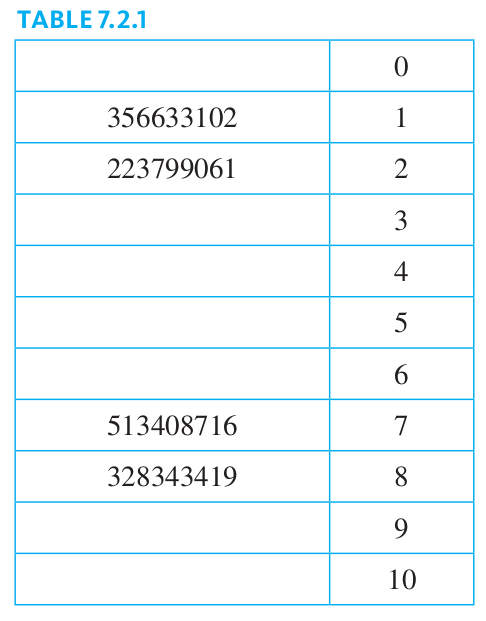
\includegraphics[scale=0.3]{../images/7.2.1.png}
\end{figure}

\subsubsection{(a)}
417302072

\begin{proof}
When 417302072 is divided by 11, the remainder is 0. So, \(417302072 \mod 11 = H(417302072) = 0\). 
Since position 0 is unoccupied, the record is placed there.
\end{proof}

\subsubsection{(b)}
364981703

\begin{proof}
When 364981703 is divided by 11, the remainder is 9. So, \(364981703 \mod 11 = H(364981703) = 9\). 
Since position 9 is unoccupied, the record is placed there.
\end{proof}

\subsubsection{(c)}
283090787

\begin{proof}
When 283090787 is divided by 11, the remainder is 1. So, \(283090787 \mod 11 = H(283090787) = 1\). Since position 1 
is occupied, the record is placed in position 3.
\end{proof}

\subsection{Exercise 20}
Define Floor\(: \R \to \Z\) by the formula Floor\((x) = \floor{x}\), for every real number $x$. 

\subsubsection{(a)}
Is Floor one-to-one? Prove or give a counterexample.

\begin{proof}
Floor is not one-to-one. \underline{Counterexample:} Floor(0) = 0 = Floor(1/2) but $0 \neq 1/2$.
\end{proof}

\subsubsection{(b)}
Is Floor onto? Prove or give a counterexample.

\begin{proof}
Floor is onto. Suppose $m \in \Z$. {\it [We must show that there exists a real number $y$ such that Floor$(y) = m$.]} 
Let $y = m$. Then Floor$(y)$ = Floor$(m) = m$ since $m$ is an integer. (Actually, Floor takes the value $m$ for all 
real numbers in the interval \(m \leq x < m + 1\).) Hence there exists a real number $y$ such that Floor$(y) = m$ 
{\it [as was to be shown].}
\end{proof}

\subsection{Exercise 21}
Let $S$ be the set of all strings of 0’s and 1’s, and define \(L: S \to \Z^{nonneg}\) by \(L(s) =\) the length of 
$s$, for every string $s$ in $S$.

\subsubsection{(a)}
Is $L$ one-to-one? Prove or give a counterexample.

\begin{proof}
$L$ is not one-to-one. \underline{Counterexample:} \(L(0) = L(1) = 1\) but $1 \neq 0$.
\end{proof}

\subsubsection{(b)}
Is $L$ onto? Prove or give a counterexample.

\begin{proof}
$L$ is onto. Suppose $n$ is a nonnegative integer. {\it [We must show that there exists a string $s$ in $S$ such that 
\(L(s) = n\).]} Let
\[
s =
\left\{
\begin{tabular}{lr}
\(\lambda\) (the null string) & if \(n = 0\) \\
\(00\ldots0\) (with $n$ 0's) & if \(n > 0\)
\end{tabular}
\right.
\]
Then \(L(s) =\) the length of $s = n$ {\it [as was to be shown].}
\end{proof}

\subsection{Exercise 22}
Let $S$ be the set of all strings of 0’s and 1’s, and define \(D: S \to \Z\) as follows: for every string $s$ in 
$S$, \(D(s) =\) the number of 1's in $s$ minus the number of 0's in $s$.

\subsubsection{(a)}
Is $D$ one-to-one? Prove or give a counterexample.

\begin{proof}
No. \underline{Counterexample:} \(D(10) = 0 = D(01)\) but \(10 \neq 01\).
\end{proof}

\subsubsection{(b)}
Is $D$ onto? Prove or give a counterexample.

\begin{proof}
Yes. Given any $n \in \Z$, if $n < 0$ then let $s$ be the string of $-n$ consecutive 0's. Then $D(s) = n$.
Similarly if $n > 0$ then let $s$ be the string of $n$ consecutive 1's. Then $D(s) = n$.
If $n = 0$ then $D(\lambda) = n$.
\end{proof}

\subsection{Exercise 23}
Define \(F: \ps(\{a, b, c\}) \to \Z\) as follows: For every
$A$ in \(\ps(\{a, b, c\})\), \(F(A) =\) the number of 
elements in $A$.

\subsubsection{(a)}
Is $F$ one-to-one? Prove or give a counterexample. 

\begin{proof}
$F$ is not one-to-one. \underline{Counterexample:} Let \(A = \{a\}, B = \{b\}\). Then \(F(A) = F(B) = 1\) but \(A \neq B\).
\end{proof}

\subsubsection{(b)}
Is $F$ onto? Prove or give a counterexample. 

\begin{proof}
No. \underline{Counterexample:} There are no subsets of $A$ with a negative number of, say, $-1$ elements.
\end{proof}

\subsection{Exercise 24}
Let $S$ be the set of all strings of $a$’s and $b$’s, and define \(N: S \to \Z\) by \(N(s) =\) the number of $a$’s in 
$s$, for each \(s \in S\).

\subsubsection{(a)}
Is $N$ one-to-one? Prove or give a counterexample. 

\begin{proof}
No. \underline{Counterexample:} $N(a) = 1 = N(ab)$ but $a \neq ab$.
\end{proof}

\subsubsection{(b)}
Is $N$ onto? Prove or give a counterexample. 

\begin{proof}
No. \underline{Counterexample:} There are no strings with $-1$ $a$'s in it.
\end{proof}

\subsection{Exercise 25}
Let $S$ be the set of all strings in $a$’s and $b$’s, and
define \(C: S \to S\) by \(C(s) = as\), for each $s \in S$.
($C$ is called concatenation by $a$ on the left.)

\subsubsection{(a)}
Is $C$ one-to-one? Prove or give a counterexample.

\begin{proof}
Yes. Assume \(C(s_1) = C(s_2)\). So \(as_1 = as_2\). Then $s_1$ and $s_2$ are the same string.
\end{proof}

\subsubsection{(b)}
Is $C$ onto? Prove or give a counterexample.

\begin{proof}
No. \underline{Counterexample:} there is no string $s$ such that \(C(s) = b\) because $b$ has no $a$'s in it.
\end{proof}

\subsection{Exercise 26}
Define \(S: \Z^+ \to \Z^+\) by the rule: For each integer $n$, $S(n) =$ the sum of the positive divisors of $n$.

\subsubsection{(a)}
Is $S$ one-to-one? Prove or give a counterexample.

\begin{proof}
No. \underline{Counterexample:} \(S(6) = 1 + 2 + 3 + 6 = 12\) and \(S(11) = 1 + 11 = 12\) but \(6 \neq 11\).
\end{proof}

\subsubsection{(b)}
Is $S$ onto? Prove or give a counterexample.

\begin{proof}
No. \underline{Counterexample:} In order for there to be a positive integer $n$ such that $S(n) = 5$, $n$ would have 
to be less than 5. But \(S(1) = 1, S(2) = 3, S(3) = 4\), and \(S(4) = 7\). Hence there is no positive integer $n$ 
such that \(S(n) = 5\).
\end{proof}

\subsection{Exercise 27}
Let $D$ be the set of all finite subsets of positive integers, and define \(T: \Z^+ \to D\) by the following 
rule: For every integer $n$, $T(n) =$ the set of all of the positive divisors of $n$.

\subsubsection{(a)}
Is $T$ one-to-one? Prove or give a counterexample.

\begin{proof}
Yes. Assume \(T(n_1) = T(n_2)\). {\it [We want to show \(n_1 = n_2\)].} Argue by contradiction and assume 
\(n_1 \neq n_2\). Then either \(n_1 < n_2\) or \(n_1 > n_2\). In the first case, $n_2$ is a positive divisor of 
$n_2$ so \(n_2 \in T(n_2)\). But since \(T(n_1) = T(n_2), n_2 \in T(n_1)\) too. So $n_2$ is a positive divisor of 
$n_1$, contradiction. The other case is similar.
\end{proof}

\subsubsection{(b)}
Is $T$ onto? Prove or give a counterexample.

\begin{proof}
No. \underline{Counterexample:} There is no \(n \in \Z^+\) such that \(T(n) = \{1, 2, 3\}\), any such $n$ would also 
be divisible by 6, so \(T(n)\) would have to include 6 too.
\end{proof}

\subsection{Exercise 28}
Define \(G: \R \times \R \to \R \times \R\) as follows: \(G(x, y) = (2y, -x)\) for every \((x, y) \in \R \times \R\).

\subsubsection{(a)}
Is $G$ one-to-one? Prove or give a counterexample.

\begin{proof}
Yes. Suppose \((x_1, y_1)\) and \((x_2, y_2)\) are any elements of \(\R \times \R\) such that \(G(x_1, y_1) = 
G(x_ 2, y_2)\). {\it [We must show that \((x_1, y_1) = (x_2, y_2)\).]} Then, by definition of $G$, \((2y_1, -x_1) 
= (2y_2, -x_2)\), and, by definition of ordered pair, \(2y_1 = 2y_2\) and \(-x_1 = -x_2\). Dividing both sides of 
the equation on the left by 2 and both sides of the equation on the right by $-1$ gives that \(y_1 = y_2\) and 
\(x_1 = x_2\), and so, by definition of ordered pair, \((x_1, y_1) = (x_2, y_2)\) {\it [as was to be shown].}
\end{proof}

\subsubsection{(b)}
Is $G$ onto? Prove or give a counterexample.

\begin{proof}
Yes. Suppose \((u, v)\) is any element of \(\R \times \R\). {\it [We must show that there is an element \((x, y)\) in 
\(\R \times \R\) such that \(G(x, y) = (u, v)\).]} Let \((x, y) = (-v, u/2)\). Then (1) \((x, y) \in \R \times \R\) 
and (2) \(G(x, y) = (2y, -x) = (2(u/2), -(-v)) = (u, v)\) {\it [as was to be shown].}
\end{proof}

\subsection{Exercise 29}
Define \(H: \R \times \R \to \R \times \R\) as follows: \(H(x, y) = (x+1, 2-y)\) for every \((x, y) \in \R \times \R\).

\subsubsection{(a)}
Is $H$ one-to-one? Prove or give a counterexample.

\begin{proof}
Yes. Assume \(H(x_1, y_1) = H(x_2, y_2)\). {\it [We want to show that \(x_1 = x_2\) and \(y_1 = y_2)\).]}
We have \((x_1+1, 2-y_1) = (x_2+1, 2-y_2)\). By definition of a tuple, \(x_1+1 = x_2+1\) and \(2-y_1 = 2-y_2\).
Solving, we get \(x_1 = x_2\) and \(y_1 = y_2)\).
\end{proof}

\subsubsection{(b)}
Is $H$ onto? Prove or give a counterexample.

\begin{proof}
Yes. Assume \((x,y) \in \R \times \R\) is any pair of real numbers. {\it [We want to show there exists a pair
\((a, b) \in \R \times \R\) such that \(H(a,b) = (x,y)\).]} Let \(a = x-1, b = 2-y\). Then \(H(a, b) = (a+1, 2-b) = 
(x-1+1, 2-(2-y)) = (x,y)\), {\it [as was to be shown.]}
\end{proof}

\subsection{Exercise 30}
Define \(J: \Q \times \Q \to \R\) as follows: \(J(r, s) = r + \sqrt{2}s\) for every \((r, s) \in \Q \times \Q\).

\subsubsection{(a)}
Is $J$ one-to-one? Prove or give a counterexample.

\begin{proof}
Yes. Assume \(J(r_1, s_1) = J(r_2, s_2)\). {\it [We want to show that \(r_1 = r_2\) and \(s_1 = s_2)\).]}
We have \(r_1 + \sqrt{2}s_1 = r_2 + \sqrt{2}s_2\). Moving terms around we get (*) \(r_1-r_2=\sqrt{2}(s_2-s_1)\).
For the moment assume \(s_1 \neq s_2\). Then \(s_2 - s_1 \neq 0\). Dividing, we get
\[
\frac{r_1 - r_2}{s_2 - s_1} = \sqrt{2}.
\]
This is a contradiction, since the right hand side is an irrational number, and the left hand side is a rational
number (being a ratio of differences of rational numbers). Thus our supposition was false and \(s_1 = s_2\). Going
back to the equation (*), this gives \(r_1-r_2=\sqrt{2} \cdot 0 = 0\) and thus \(r_1 = r_2\), as was to be shown.
\end{proof}

\subsubsection{(b)}
Is $J$ onto? Prove or give a counterexample.

\begin{proof}
No. \underline{Counterexample:} There are no rationals $(r, s)$ such that \(J(r,s) = \sqrt{3}\). Argue by contradiction
and assume \(J(r,s) = \sqrt{3}\) for some rationals $r,s$. Then \(r + \sqrt{2}s = \sqrt{3}\). Squaring both sides, we
get 
\[
(r + \sqrt{2}s)^2 = \sqrt{3}^2 \implies r^2 + 2rs\sqrt{2} + 2s^2 = 3 \implies \sqrt{2} = \frac{3 - r^2 - 2s^2}{2rs}.
\]
This is a contradiction, since the left hand side is irrational, and the right side is rational (being a ratio 
of differences of products of rationals). Thus our supposition was false, and $J$ is not onto.
\end{proof}

\subsection{Exercise 31}
Define \(F: \Z^+ \times \Z^+ \to \Z^+\) and \(G: \Z^+ \times \Z^+ \to \Z^+\) as follows: for each \((n, m) \in 
\Z^+ \times \Z^+, F(n, m) = 3^n5^m\) and \(G(n, m) = 3^n6^m\).

\subsubsection{(a)}
Is $F$ one-to-one? Prove or give a counterexample.

\begin{proof}
Yes. Assume \(F(n_1, m_1) = F(n_2, m_2)\). Then \(3^{n_1}5^{m_1} = 3^{n_2}5^{n_2}\). Call this positive integer $z$.
So we have two different prime factorizations of the same integer $z$. By the uniqueness part of the factorization
theorem, the exponents are unique, therefore \(n_1 = n_2\) and \(m_1 = m_2\).
\end{proof}

\subsubsection{(b)}
Is $G$ one-to-one? Prove or give a counterexample.

\begin{proof}
Yes. We can rewrite \(G(n, m) = 3^n6^m = 3^n (2 \cdot 3)^m = 3^n \cdot 2^m \cdot 3^m = 2^m \cdot 3^{m+n}\). Now 
assume \(G(n_1, m_1) = G(n_2, m_2)\). Then \(2^{m_1} \cdot 3^{m_1+n_1} = 2^{m_2} \cdot 3^{m_2+n_2}\). Similar to part
(a), by the uniqueness of prime factorizations, the exponents must be equal, so \(m_1 = m_2\) and 
\(m_1 + n_1 = m_2 + n_2\). Using \(m_1 = m_2\) in the second equation we can cancel the $m$s to get \(n_1=n_2\).
\end{proof}

\subsection{Exercise 32}
\subsubsection{(a)}
Is \(\log_8 27 = \log_2 3\)? Why or why not?

\begin{proof}
1. Let \(x = \log_8 27, y = \log_2 3\).

2. By 1 and definition of logarithm, \(8^x = 27\) and \(2^y = 3\).

3. By 2 and laws of exponents, \((2^3)^x = 2^{3x} = (2^x)^3\) and \(27 = 3^3\). So \((2^x)^3 = 3^3\).

4. By 3, taking the cube root of both sides, we get \(2^x = 3\).

5. By 2 and 4, \(2^x = 2^y\). Applying \(\log_2\) to both sides, we get $x = y$.
\end{proof}

\subsubsection{(b)}
Is \(\log_{16} 9 = \log_4 3\)? Why or why not?

\begin{proof}
1. Let \(x = \log_{16} 9, y = \log_4 3\).

2. By 1 and definition of logarithm, \(16^x = 9\) and \(4^y = 3\).

3. By 2 and laws of exponents, \((2^4)^x = 2^{4x} = (2^{2x})^2\) and \(9 = 3^2\). So \((2^{2x})^2 = 3^2\).
Similarly \(2^{2y} = 3\).

4. By 3, taking the square root of both sides, we get \(2^{2x} = 3\).

5. By 2 and 4, \(2^{2x} = 2^{2y}\). Applying \(\log_2\) to both sides, we get $2x = 2y$ so $x = y$.
\end{proof}

{\bf \cy The properties of logarithm established in $33-35$ are used in Sections 11.4 and 11.5.}

\subsection{Exercise 33}
Prove that for all positive real numbers $b$, $x$, and $y$ with \(b \neq 1\),
\[
\log_b\left(\frac{x}{y}\right) = \log_b x - \log_b y.
\]
\begin{proof}
Suppose that $b$, $x$, and $y$ are any positive real numbers such that \(b \neq 1\). Let \(u = \log_b(x)\) and 
\(v = \log_b(y)\). By definition of logarithm, \(b^u = x\) and \(b_v = y\). By substitution, \(\frac{x}{y} = 
\frac{b^u}{b^v} = b^{u-v}\) {\it [by (7.2.3) and the fact that \(b^{-v} = \frac{1}{b^v}\)].} Translating 
\(\frac{x}{y} = b^{u-v}\) into logarithmic form gives \(\log_b \frac{x}{y} = u-v\), and so, by substitution, 
\(\log_b \frac{x}{y} = \log_b(x) - \log_b(y)\), {\it [as was to be shown].}
\end{proof}

\subsection{Exercise 34}
Prove that for all positive real numbers $b$, $x$, and $y$ with \(b \neq 1\),
\[
\log_b(xy) = \log_b x + \log_b y.
\]
\begin{proof}
1. Let \(z = \log_b(xy), m = \log_b x, n = \log_b y\).

2. By 1 and definition of log, \(b^z = xy\).

3. By 1 and definition of log, \(b^m = x\).

4. By 1 and definition of log, \(b^n = y\).

5. By 2, 3, 4, and law of exponents, \(b^z = xy = b^m \cdot b^n = b^{m+n}\).

6. By 5, applying $\log_b$ to both sides, we get \(\log_b(b^z) = \log_b(b^{m+n})\), which gives $z = m+n$.

7. By 1 and 6, \(\log_b(xy) = \log_b x + \log_b y\).
\end{proof}

\subsection{Exercise 35}
Prove that for all real numbers $a$, $b$ and $x$ with $b$ and $x$ positive and \(b \neq 1\),
\[
\log_b (x^a) = a \log_b x.
\]
\begin{proof}
1. Let \(z = \log_b(x^a), m = \log_b x\).

2. By 1 and definition of log, \(b^z = x^a\).

3. By 1 and definition of log, \(b^m = x\).

4. By 3 and law of exponents, \((b^m)^a = x^a\) so \(b^{am} = x^a\).

5. By 2 and 4, \(b^z = x^a = b^{am}\).

6. By 5, applying $\log_b$ to both sides, we get \(\log_b(b^z) = \log_b(b^{am})\), which gives $z = am$.

7. By 1 and 6, \(\log_b(x^a) = a \log_b x\).
\end{proof}

{\bf \cy Exercises 36 and 37 use the following definition: If \(f: \R \to \R\) and \(g: \R \to \R\) are functions, 
then the function \((f + g): \R \to \R\) is defined by the formula \((f + g)(x) = f(x) + g(x)\) for every real number $x$.}

\subsection{Exercise 36}
If \(f: \R \to \R\) and \(g: \R \to \R\) are both one-to-one, is \(f + g\) also one-to-one? Justify your answer.

\begin{proof}
No. \underline{Counterexample:} Define \(f: \R \to \R\) and \(g: \R \to \R\) as follows: \(f(x) = x\) and \(g(x) = -x\) 
for every real number $x$. Then $f$ and $g$ are both one-to-one {\it [because for all real numbers $x_1$ and $x_2$, 
if \(f(x_1) = f(x_2)\) then \(x_1 = x_2\), and if \(g(x_1) = g(x_2)\) then \(-x_1 = -x_2\), so \(x_1 = x_2\) in this 
case as well].} But \(f + g\) is not one-to-one {\it [because $f + g$ satisfies the equation \((f + g)(x) = x + 
(-x) = 0\) for every real number $x$, and so, for instance, \((f + g)(1) = (f + g)(2)\) but $1 \neq 2$].}
\end{proof}

\subsection{Exercise 37}
If \(f: \R \to \R\) and \(g: \R \to \R\) are both onto, is \(f + g\) also onto? Justify your answer.

\begin{proof}
No. Same counterexample as exercise 36 works. \(f(x) = x\) and \(g(x) = -x\) are both onto, but \((f+g)(x) = 0\) is not.
\end{proof}

{\bf \cy Exercises 38 and 39 use the following definition: If \(f: \R \to \R\) is a function and $c$ is a nonzero real 
number, then the function \((c \cdot f): \R \to \R\) is defined by the formula \((c \cdot f)(x) = c \cdot (f(x))\) 
for every real number $x$.}

\subsection{Exercise 38}
Let \(f: \R \to \R\) be a function and $c$ a nonzero real number. If $f$ is one-to-one, is \(c \cdot f\) also one-to-
one? Justify your answer.

\begin{proof}
Yes. Let $f$ be a one-to-one function from $\R$ to $\R$, and let $c$ be any nonzero real number. Suppose 
\((c \cdot f)(x_1) = (c \cdot f)(x_2)\). {\it [We must show that \(x_1 = x_2\).]} It follows by definition of 
\((c \cdot f)\) that \(c \cdot (f(x1)) = c \cdot (f(x_2))\). Since \(c \neq 0\), we may divide both sides of the 
equation by $c$ to obtain \(f(x_1) = f(x_2)\). And since $f$ is one-to-one, this implies that \(x_1 = x_2\), 
{\it [as was to be shown].}
\end{proof}

\subsection{Exercise 39}
Let \(f: \R \to \R\) be a function and $c$ a nonzero real number. If $f$ is onto, is \(c \cdot f\) also onto? 
Justify your answer.

\begin{proof}
Yes. Suppose \(y \in \R\). {\it [We want to show there exists \(x \in \R\) such that \((c \cdot f)(x) = y\)].}
Since \(c \neq 0\) and $f$ is onto, there exists \(z \in \R\) such that \(f(z) = y/c\). Let $x = z$. Then 
\((c \cdot f)(x) = c \cdot f(x) = c \cdot f(z) = c \cdot (y/c) = y\), {\it [as was to be shown]}.
\end{proof}

\subsection{Exercise 40}
Suppose \(F: X \to Y\) is one-to-one.

\subsubsection{(a)}
Prove that for every subset \(A \subseteq X, F^{-1}(F(A)) = A\).

\begin{proof}
Assume \(A \subseteq X\).

1. Assume \(x \in F^{-1}(F(A))\). {\it [Want to show \(x \in A\).]}

2. By 1 and definition of inverse image \(F^{-1}(F(A)) = \{t \in X \, | \, F(t) \in F(A)\}\) applied to $t = x$, we have \(x \in X\) and \(F(x) \in F(A)\).

3. By 2 and definition of $F(A)$, there exists \(r \in A\) such that \(F(r) = F(x)\).

4. By 3 and since $F$ is 1-1, $r = x$, hence \(x \in A\).

5. By 1, 4 and definition of subset, \(F^{-1}(F(A)) \subseteq A\).

{\it Now the reverse direction:}

6. Assume \(x \in A\). {\it [Want to show \(x \in F^{-1}(F(A))\).]}

7. By 6 and definition of $F(A)$, we have \(F(x) \in F(A)\).

8. By 6 and 7, \(x \in X\) and \(F(x) \in F(A)\). So $x$ satisfies the definition of being a member of the inverse 
image \(F^{-1}(F(A)) = \{t \in X \, | \, F(t) \in F(A)\}\) (with $t = x$). Therefore we have \(x \in F^{-1}(F(A))\).

9. By 6, 8 and definition of subset, \(A \subseteq F^{-1}(F(A))\).

{\it Conclusion:}

10. By 5, 9 and definition of set equality, \(F^{-1}(F(A)) = A\).
\end{proof}

\subsubsection{(b)}
Prove that for all subsets $A_1$ and $A_2$ in $X$, \(F(A_1 \cap A_2) = F(A_1) \cap F(A_2)\).

\begin{proof}
Assume \(A_1 \subseteq X, A_2 \subseteq X\).

1. Assume \(y \in F(A_1 \cap A_2)\). {\it [Want to show \(y \in F(A_1) \cap F(A_2)\).]}

2. By 1 and definition of \(F(A_1 \cap A_2)\), there exists \(x \in A_1 \cap A_2\) such that \(y = F(x)\).

3. By 2 and definition of intersection, \(x \in A_1\) and \(x \in A_2\).

4. By 3, and since $y = F(x)$, and by definitions of $F(A_1)$ and $F(A_2)$, \(y \in F(A_1)\) and \(y \in F(A_2)\).

5. By 4 and definition of intersection, \(y \in F(A_1) \cap F(A_2)\).

6. By 1, 5 and definition of subset, \(F(A_1 \cap A_2) \subseteq F(A_1) \cap F(A_2)\).

{\it Now the reverse direction:}

7. Assume \(y \in F(A_1) \cap F(A_2)\). {\it [Want to show \(y \in F(A_1 \cap A_2)\).]}

8. By 7 and definition of intersection, \(y \in F(A_1)\) and \(y \in F(A_2)\).

9. By 8 and definitions of \(F(A_1)\) and \(F(A_2)\), there exist \(x_1 \in A_1\) and \(x_2 \in A_2\) such that \(y = F(x_1)\) and \(y = F(x_2)\).

10. By 9 and since $F$ is 1-1, \(x_1 = x_2\). 

11. By 9, 10 and definition of intersection, \(x_1 \in A_1 \cap A_2\).

12. By 11 and since \(y = F(x_1), y \in F(A_1 \cap A_2)\).

13. By 7, 12 and definition of subset, \(F(A_1) \cap F(A_2) \subseteq F(A_1 \cap A_2)\).

{\it Conclusion:}

14. By 6, 13 and definition of set equality, \(F(A_1 \cap A_2) = F(A_1) \cap F(A_2)\).
\end{proof}

\subsection{Exercise 41}
Suppose \(F: X \to Y\) is onto. Prove that for every subset \(B \subseteq Y, F(F^{-1}(B)) = B\).

\begin{proof}
Assume \(B \subseteq Y\).

1. Assume \(y \in F(F^{-1}(B))\). {\it [Want to show \(y \in B\).]}

2. By 1 and definition of \(F(F^{-1}(B))\), there exists \(x \in F^{-1}(B)\) such that \(F(x) = y\).

3. By 2 and definition of inverse image \(F^{-1}(B) = \{t \in X \, | \, F(t) \in B\}\), we have \(F(x) \in B\).

4. By 2 and 3, \(y = F(x) \in B\). So \(y \in B\).

5. By 1, 4 and definition of subset, \(F(F^{-1}(B)) \subseteq B\).

{\it Now the reverse direction:}

6. Assume \(y \in B\). {\it [Want to show \(y \in F(F^{-1}(B))\).]}

7. By 6 and since $F$ is onto, there exists \(x \in X\) such that \(F(x) = y\).

8. By 6 and 7, \(x \in X\) and \(F(x) \in B\). So $x$ satisfies the definition of being a member of the inverse
image \(F^{-1}(B) = \{t \in X \, | \, F(t) \in B\}\) (with $t = x$). So \(x \in F^{-1}(B)\).

9. By 7 and 8, \(y = F(x) \in F(F^{-1}(B))\).

10. By 6, 9 and definition of subset, \(B \subseteq F(F^{-1}(B))\).

{\it Conclusion:}

11. By 5, 10 and definition of set equality, \(F(F^{-1}(B)) = B\).
\end{proof}

{\bf \cy Let \(X = \{a, b, c, d, e\}\) and \(Y = \{s, t, u, v, w\}\). In each of 42 and 43 a one-to-one correspondence 
\(F: X \to Y\) is defined by an arrow diagram. In each case draw an arrow diagram for \(F^{-1}\).}

\subsection{Exercise 42}
\begin{figure}[ht!]
\centering
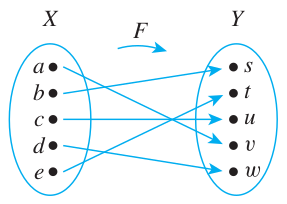
\includegraphics[scale=0.8]{../images/7.2.42.png}
\end{figure}

\begin{proof}
\begin{figure}[ht!]
\centering
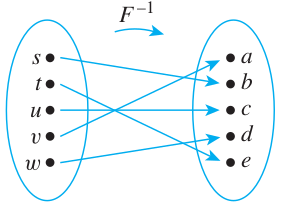
\includegraphics[scale=0.5]{../images/7.2.42.sol.png}
\end{figure}
\end{proof}

\subsection{Exercise 43}
\begin{figure}[ht!]
\centering
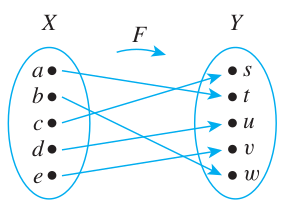
\includegraphics[scale=0.5]{../images/7.2.43.png}
\end{figure}

\begin{proof}
\begin{figure}[ht!]
\centering
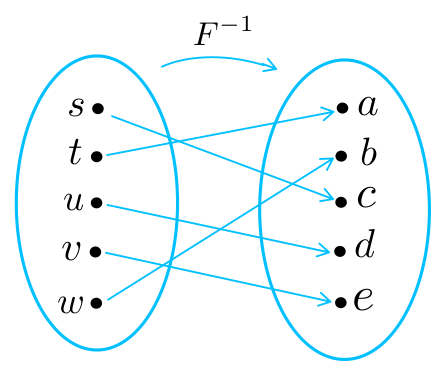
\includegraphics[scale=0.4]{../images/7.2.43.sol.png}
\end{figure}
\end{proof}

{\bf \cy In $44-55$ indicate which of the functions in the referenced exercise are one-to-one correspondences. For 
each function that is a one-to-one correspondence, find the inverse function.}

\subsection{Exercise 44}
Exercise 10a
\begin{proof}
The function is not a one-to-one correspondence because it is not onto.
\end{proof}

\subsection{Exercise 45}
Exercise 10b
\begin{proof}
The answer to exercise 10(b) shows that $h$ is onto. To show that $h$ is one-to-one, suppose \(h(n_1) = h(n_2)\). 
By definition of $h$, this implies that \(2n_1 = 2n_2\). Dividing both sides by 2 gives \(n_1 = n_2\). Hence $h$ is 
one-to-one, and so $h$ is a one-to-one correspondence. Given any even integer $m$, if \(m = h(n)\), then by 
definition of \(h, m = 2n\), and so \(n = m/2\). Thus \(h^{-1}(m) = m/2\) for every \(m \in 2\Z\).
\end{proof}

\subsection{Exercise 46}
Exercise 11a
\begin{proof}
The function $g$ is not a one-to-one correspondence because it is not onto. For instance, if $m = 2$, it is impossible 
to find an integer $n$ such that \(g(n) = m\). (This is because if \(g(n) = m\), then \(4n - 5 = 2\), which implies 
that \(n = 7/4\). Thus the only number $n$ with the property that \(g(n) = m\) is 7/4. But 7/4 is not an integer.)
\end{proof}

\subsection{Exercise 47}
Exercise 11b
\begin{proof}
The answer to exercise 11b shows that $G$ is onto. In addition, $G$ is one-to-one. To prove this, suppose 
\(G(x_1) = G(x_2)\) for some $x_1$ and $x_2$ in $\R$. {\it [We must show that \(x_1 = x_2\).]} By definition of $G$, 
\(4x_1 - 5 = 4x_2 - 5\). Add 5 to both sides of this equation and divide both sides by 4 to obtain \(x_1 = x_2\) 
{\it [as was to be shown]}. We claim that \(G^{-1}(y) = (y + 5)/4\) for each $y$ in $\R$. By definition of inverse 
function, this is true if, and only if, \(G((y + 5)/4) = y\). But \(G((y+5)/4) = 4((y + 5)/4)-5=(y + 5) - 5 = y\), 
and so it is the case that \(G^{-1}(y) = (y + 5)/4\) for each $y$ in $\R$.
\end{proof}

\subsection{Exercise 48}
Exercise 12a
\begin{proof}
The function $F$ is not a one-to-one correspondence because it is not onto.
\end{proof}

\subsection{Exercise 49}
Exercise 12b
\begin{proof}
The function $G$ is a one-to-one correspondence because it is both one-to-one and onto. As shown in the solution to
exercise 12b, the inverse function is \(G^{-1}(y) = \frac{y-2}{-3}\).
\end{proof}

\subsection{Exercise 50}
Exercise 21
\begin{proof}
The function $L$ is not a one-to-one correspondence because it is not 1-1.
\end{proof}

\subsection{Exercise 51}
Exercise 22
\begin{proof}
The function $D$ is not a one-to-one correspondence because it is not 1-1.
\end{proof}

\subsection{Exercise 52}
Exercise 15 with the co-domain taken to be the set of all real numbers not equal to 1

\begin{proof}
The answer to exercise 15 shows that $f$ is one-to-one, and if the co-domain is taken to be the set of all real numbers 
not equal to 1, then $f$ is also onto. The reason is that given any real number \(y \neq 1\), if we take 
\(x = \frac{1}{y-1}\), then $x$ is a real number and
\[
f(x) = f\left(\frac{1}{y-1}\right) = \frac{\frac{1}{y-1} + 1}{\frac{1}{y-1}} = \frac{1+(y-1)}{1} = y.
\]
Thus \(f^{-1}(y) = \frac{1}{y-1}\) for each real number \(y \neq 1\).
\end{proof}

\subsection{Exercise 53}
Exercise 16 with the co-domain taken to be the set of all real numbers

\begin{proof}
The answer to exercise 16 shows that $f$ is not one-to-one. Therefore, it is not a one-to-one correspondence.
\end{proof}

\subsection{Exercise 54}
Exercise 17 with the co-domain taken to be the set of all real numbers not equal to 3

\begin{proof}
The answer to exercise 17 shows that $f$ is 1-1. If the co-domain excludes 3, then it also becomes onto. Assume $y$ is
any real number with \(y \neq 3\). Then letting \(y = \frac{3x-1}{x}\) and solving, we get \(x = \frac{1}{3-y}\)
which is defined since \(y \neq 3\). Thus $f$ is a one-to-one correspondence and \(f^{-1}(y) = \frac{1}{3-y}\).
\end{proof}

\subsection{Exercise 55}
Exercise 18 with the co-domain taken to be the set of all real numbers not equal to 1

\begin{proof}
The answer to exercise 18 shows that $f$ is 1-1. If the co-domain excludes 1, then it also becomes onto. Assume $y$ is
any real number with \(y \neq 1\). Then letting \(y = \frac{x+1}{x-1}\) and solving, we get \(x=\frac{y+1}{y-1}\) 
which is defined since \(y \neq 1\). Thus $f$ is a one-to-one correspondence and \(f^{-1}(y) = \frac{y+1}{y-1}\).
\end{proof}

\subsection{Exercise 56}
In Example 7.2.8 a one-to-one correspondence was defined from the power set of $\{a, b\}$ to the set of all strings 
of 0’s and 1’s that have length 2. Thus the elements of these two sets can be matched up exactly, and so the two 
sets have the same number of elements.

\subsubsection{(a)}
Let \(X = \{x_1, x_2 , \ldots, x_n\}\) be a set with $n$ elements. Use Example 7.2.8 as a model to define a 
one-to-one correspondence from \(\ps(X)\), the set of all subsets of $X$, to the set of all strings of 0’s and 1’s 
that have length $n$.

\begin{proof}
Let $S_n$ be the set of all strings of 0's and 1's that have length $n$. 

Define \(f : \ps(X) \to S_n\) as follows. For any subset $A$ of $X$, define $f(A)$ to be the string where, the $n$th 
character in the string is 0 if \(x_i \notin A\), and 1 if \(x_i \in A\).

For example, if $n=5$ and \(A = \{x_2, x_4\}\) then \(f(A) = 01010\).
\end{proof}

\subsubsection{(b)}
In Section 9.2 we show that there are $2^n$ strings of 0’s and 1’s that have length $n$. What does this allow you to 
conclude about the number of elements of $\ps(X)$? (This provides an alternative proof of Theorem 6.3.1.)

\begin{proof}
Since \(f: \ps(X) \to S_n\) is a one-to-one correspondence, \(\ps(X)\) has the same number of elements as \(S_n\). 
Since \(S_n\) has $2^n$ elements, $\ps(X)$ also has $2^n$ elements.
\end{proof}

\subsection{Exercise 57}
Write a computer algorithm to check whether a function from one finite set to another is one-to-one. Assume the 
existence of an independent algorithm to compute values of the function.

\begin{proof}
Let a function $F$ be given and suppose the domain of $F$ is represented as a one-dimensional array 
\(a[1], a[2], \ldots, a[n]\). 

\begin{tabbing}
\(answer \coloneqq\) ``one-to-one'' \\
\(i \coloneqq 1\) \\
{\bf while} \= (\(i \leq n-1\) and \(answer = \) ``one-to-one'') \\
            \> \(j \coloneqq i + 1\) \\
            \> {\bf while} \= (\(j \leq n\) and \(answer =\) ''one-to-one'') \\
            \>             \> {\bf if} (\(F(a[i]) = F(a[j])\) and \(a[i] \neq a[j]\)) \\
            \>             \> {\bf then} \(answer \coloneqq \) ``not one-to-one'' \\
            \>             \> \(j \coloneqq j + 1\) \\
            \> {\bf end while} \\
\(i \coloneqq i + 1\) \\
{\bf end while} \\
{\bf return} $answer$
\end{tabbing}
\end{proof}

\subsection{Exercise 58}
Write a computer algorithm to check whether a function from one finite set to another is onto. Assume the existence of 
an independent algorithm to compute values of the function.

\begin{proof}
Let a function $F$ be given and suppose the domain and the co-domain of $F$ are represented as one-dimensional arrays 
\(a[1], a[2], \ldots, a[n]\) and \(b[1], b[2], \ldots, b[m]\).

\begin{tabbing}
\(answer \coloneqq\) ``onto'' \\
\(i \coloneqq 1\) \\
{\bf while} \= (\(i\leq m\) and \(answer = \) ``onto'') \\
            \> \(found \coloneqq\) ``false'' \\
            \> \(j \coloneqq 1\) \\
            \> {\bf while} \= (\(j \leq n\) and \(found =\) ``false'') \\
            \>             \> {\bf if} (\(b[i]=F(a[j])\))\\
            \>             \> {\bf then} \(found \coloneqq \) ``true'' \\
            \>             \> \(j \coloneqq j + 1\) \\
            \> {\bf end while} \\
            \> {\bf if} \(found = \) false \\
            \> {\bf then} \(answer = \) ``not onto'' \\
\(i \coloneqq i + 1\) \\
{\bf end while} \\
{\bf return} $answer$
\end{tabbing}
\end{proof}

\end{document}

\section{Exercise Set 7.3}

\subsection{Exercise 1}

\begin{proof}

\end{proof}

\subsection{Exercise 2}

\begin{proof}

\end{proof}

\subsection{Exercise 3}

\begin{proof}

\end{proof}

\subsection{Exercise 4}

\begin{proof}

\end{proof}

\subsection{Exercise 5}

\begin{proof}

\end{proof}

\subsection{Exercise 6}

\begin{proof}

\end{proof}

\subsection{Exercise 7}

\begin{proof}

\end{proof}

\subsection{Exercise 8}

\begin{proof}

\end{proof}

\subsection{Exercise 9}

\begin{proof}

\end{proof}

\subsection{Exercise 10}

\begin{proof}

\end{proof}

\subsection{Exercise 11}

\begin{proof}

\end{proof}

\subsection{Exercise 12}

\begin{proof}

\end{proof}

\subsection{Exercise 13}

\begin{proof}

\end{proof}

\subsection{Exercise 14}

\begin{proof}

\end{proof}

\subsection{Exercise 15}

\begin{proof}

\end{proof}

\subsection{Exercise 16}

\begin{proof}

\end{proof}

\subsection{Exercise 17}

\begin{proof}

\end{proof}

\subsection{Exercise 18}

\begin{proof}

\end{proof}

\subsection{Exercise 19}

\begin{proof}

\end{proof}

\subsection{Exercise 20}

\begin{proof}

\end{proof}

\subsection{Exercise 21}

\begin{proof}

\end{proof}

\subsection{Exercise 22}

\begin{proof}

\end{proof}

\subsection{Exercise 23}

\begin{proof}

\end{proof}

\subsection{Exercise 24}

\begin{proof}

\end{proof}

\subsection{Exercise 25}

\begin{proof}

\end{proof}

\subsection{Exercise 26}

\begin{proof}

\end{proof}

\subsection{Exercise 27}

\begin{proof}

\end{proof}

\subsection{Exercise 28}

\begin{proof}

\end{proof}

\subsection{Exercise 29}

\begin{proof}

\end{proof}

\subsection{Exercise 30}

\begin{proof}

\end{proof}

\section{Exercise Set 7.4}

\subsection{Exercise 1}

\begin{proof}

\end{proof}

\subsection{Exercise 2}

\begin{proof}

\end{proof}

\subsection{Exercise 3}

\begin{proof}

\end{proof}

\subsection{Exercise 4}

\begin{proof}

\end{proof}

\subsection{Exercise 5}

\begin{proof}

\end{proof}

\subsection{Exercise 6}

\begin{proof}

\end{proof}

\subsection{Exercise 7}

\begin{proof}

\end{proof}

\subsection{Exercise 8}

\begin{proof}

\end{proof}

\subsection{Exercise 9}

\begin{proof}

\end{proof}

\subsection{Exercise 10}

\begin{proof}

\end{proof}

\subsection{Exercise 11}

\begin{proof}

\end{proof}

\subsection{Exercise 12}

\begin{proof}

\end{proof}

\subsection{Exercise 13}

\begin{proof}

\end{proof}

\subsection{Exercise 14}

\begin{proof}

\end{proof}

\subsection{Exercise 15}

\begin{proof}

\end{proof}

\subsection{Exercise 16}

\begin{proof}

\end{proof}

\subsection{Exercise 17}

\begin{proof}

\end{proof}

\subsection{Exercise 18}

\begin{proof}

\end{proof}

\subsection{Exercise 19}

\begin{proof}

\end{proof}

\subsection{Exercise 20}

\begin{proof}

\end{proof}

\subsection{Exercise 21}

\begin{proof}

\end{proof}

\subsection{Exercise 22}

\begin{proof}

\end{proof}

\subsection{Exercise 23}

\begin{proof}

\end{proof}

\subsection{Exercise 24}

\begin{proof}

\end{proof}

\subsection{Exercise 25}

\begin{proof}

\end{proof}

\subsection{Exercise 26}

\begin{proof}

\end{proof}

\subsection{Exercise 27}

\begin{proof}

\end{proof}

\subsection{Exercise 28}

\begin{proof}

\end{proof}

\subsection{Exercise 29}

\begin{proof}

\end{proof}

\subsection{Exercise 30}

\begin{proof}

\end{proof}

\subsection{Exercise 31}

\begin{proof}

\end{proof}

\subsection{Exercise 32}

\begin{proof}

\end{proof}

\subsection{Exercise 33}

\begin{proof}

\end{proof}

\subsection{Exercise 34}

\begin{proof}

\end{proof}

\subsection{Exercise 35}

\begin{proof}

\end{proof}

\subsection{Exercise 36}

\begin{proof}

\end{proof}

\subsection{Exercise 37}

\begin{proof}

\end{proof}

\subsection{Exercise 38}

\begin{proof}

\end{proof}

\end{document}
